\PassOptionsToPackage{table}{xcolor}
\documentclass{cernatsnote}
\usepackage[colorinlistoftodos]{todonotes}
\usepackage{placeins}
\usepackage{float}
\usepackage{rotating}
\usepackage{pdflscape}
\usepackage{verbatim}
\usepackage{fancyvrb}
\usepackage{listings}
\usepackage[T1]{fontenc}
\usepackage{graphicx}
\graphicspath{{images/}}
\usepackage{subcaption}
\usepackage{xcolor}
\usepackage{colortbl}
\usepackage{booktabs}
\usepackage{longtable}
\usepackage{multirow}
\usepackage{array}
\usepackage{listings}
\usepackage{algorithm}
\usepackage{algpseudocode}
\usepackage{xurl}   % allow long URLs (e.g. commit hashes) to break across lines
\setlength{\emergencystretch}{3em}  % absorb otherwise-overfull lines (long \texttt tokens)
\lstdefinestyle{python}{
  language=Python,
  basicstyle=\small\ttfamily,
  keywordstyle=\color[RGB]{0,0,200}\bfseries,
  stringstyle=\color[RGB]{163,21,21},
  commentstyle=\color[RGB]{0,128,0}\itshape,
  numberstyle=\tiny\color{gray},
  frame=single,
  framerule=0.4pt,
  showstringspaces=false,
  breaklines=true,
  morekeywords={True,False,None},
}

\title{DFX4ML-ARCH (Progress Update 19-5-26)}
\author{
	Omitted for blind review \\
	CERN, CH-1211 Geneva, Switzerland
}
\email{Tanawin1701d@outlook.com}
\date{\today}

\begin{document}
\maketitle

\begin{abstract}
\end{abstract}

\noindent\textit{Disclaimer: Claude (Anthropic) was used as an AI assistant in
the preparation of this report, including drafting and editing text, generating
figures, and writing supporting code. All results, figures, and conclusions were
reviewed and verified by the author.}
\bigskip

\tableofcontents

\pagebreak

\section{Architecture Upgrade}

\subsection{Dedicated Memory Transfer Ports}

Since we expect that the region may reconfiguring while inference data may also transfering, we then upgrade the system's memory transfer port to have its own dedicated port connected to the processor(PS), as shown in Figure~\ref{fig:mem_access_upgrade}.

\begin{figure}[H]
  \centering
  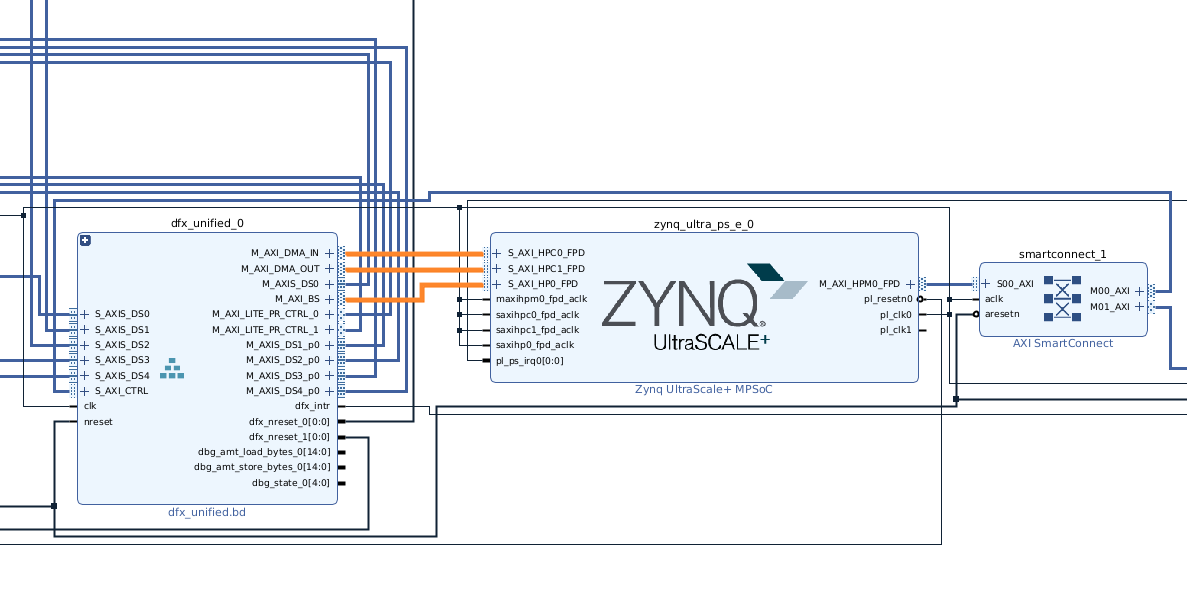
\includegraphics[width=\linewidth]{mem_access_upgrade.png}
  \caption{Memory access upgrade: a dedicated PS port for inference data transfer.}
  \label{fig:mem_access_upgrade}
\end{figure} 

For data transfering, there are 3 dedicated port as followed:

\begin{enumerate}
  \item M\_AXI\_DMA\_IN  : for DFX streamer 0 to load data to the partial region for ML inferencing.
  \item M\_AXI\_DMA\_OUT : for DFX streamer 0 to store data to the partial region for ML inferencing.
  \item M\_AXI\_BS       : for reconfiguring the partial region.
\end{enumerate}

\subsection{DFX streamer reusable in multiple region}

A single DFX streamer can be shared across multiple reconfigurable regions, loading data into each region as needed, as shown in Figure~\ref{fig:dfx_streamer_multi_load}. However, the streamer can only transfer to single region at a time.

\begin{figure}[H]
  \centering
  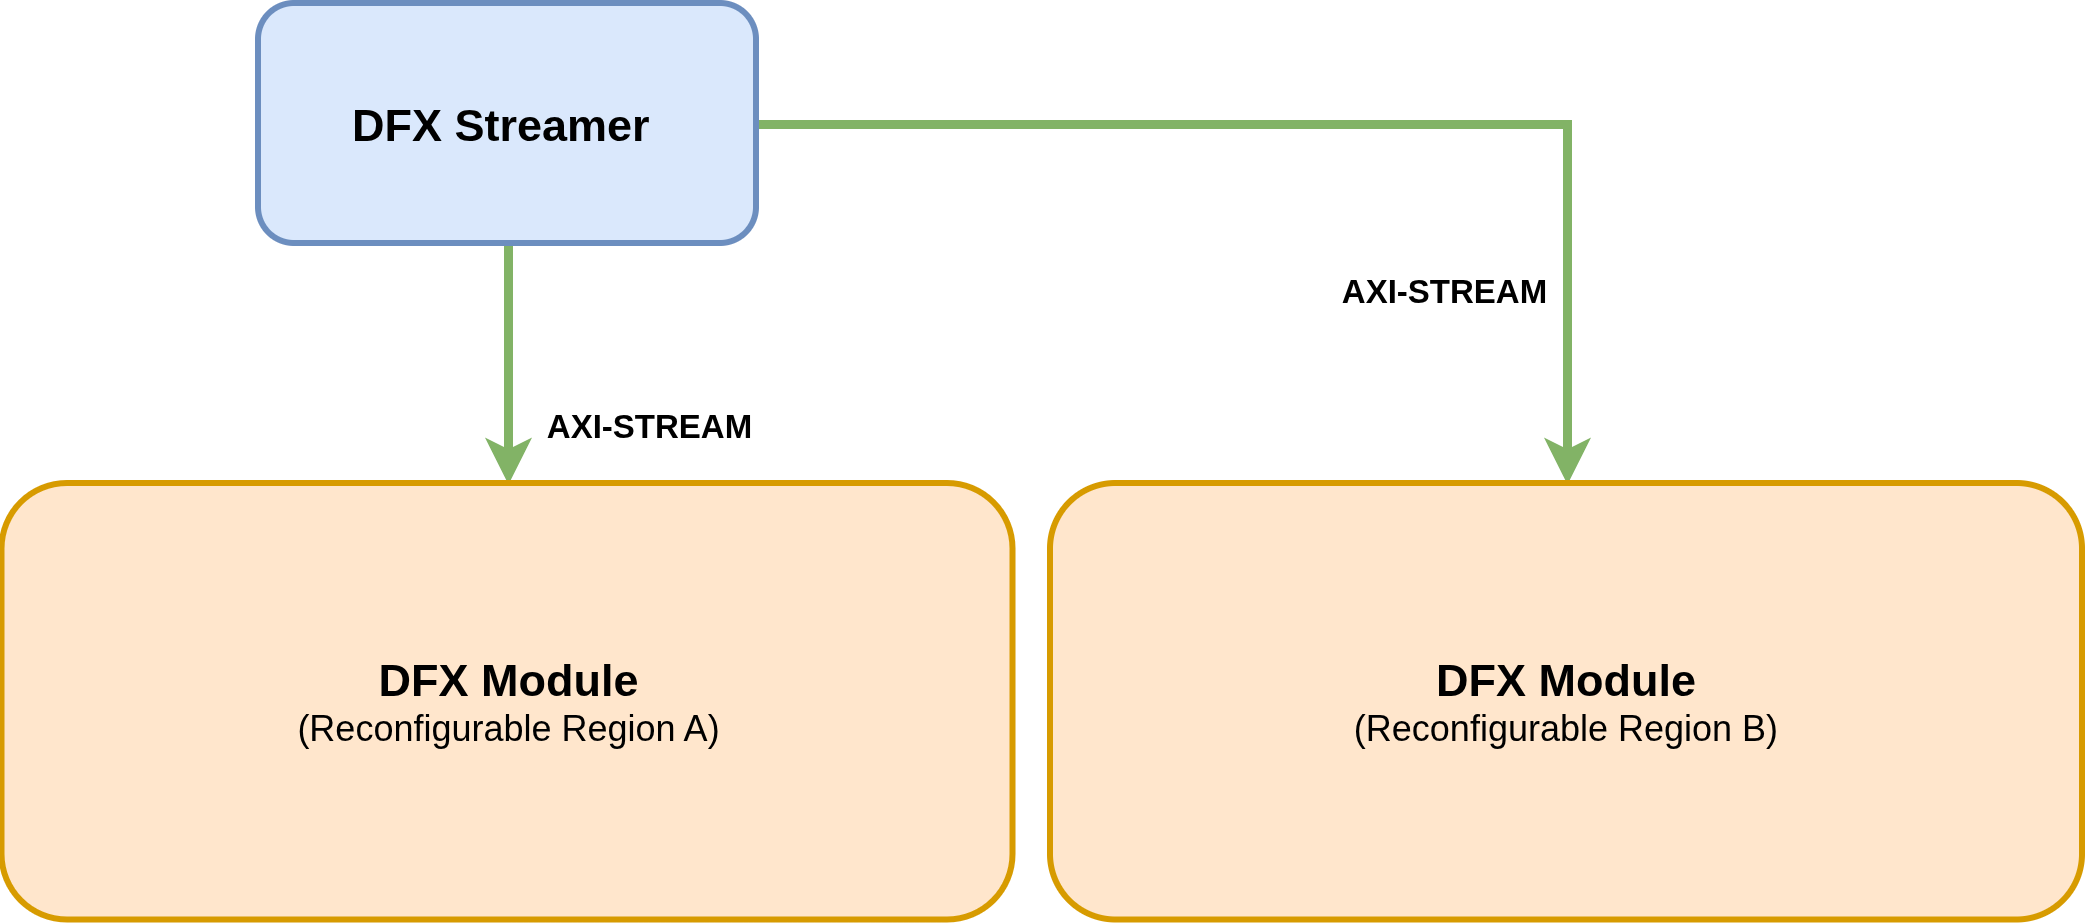
\includegraphics[width=\linewidth]{dfx_streamer_multi_load.png}
  \caption{A single DFX streamer reused to load data across multiple reconfigurable regions.}
  \label{fig:dfx_streamer_multi_load}
\end{figure}


\section{Experiment Setup}

\subsection{Model Architecture}

To test the performance in the practical use-case, we apply the U-Net architecture for this section, as shown in Figure~\ref{fig:model_full}.

\begin{figure}[H]
  \centering
  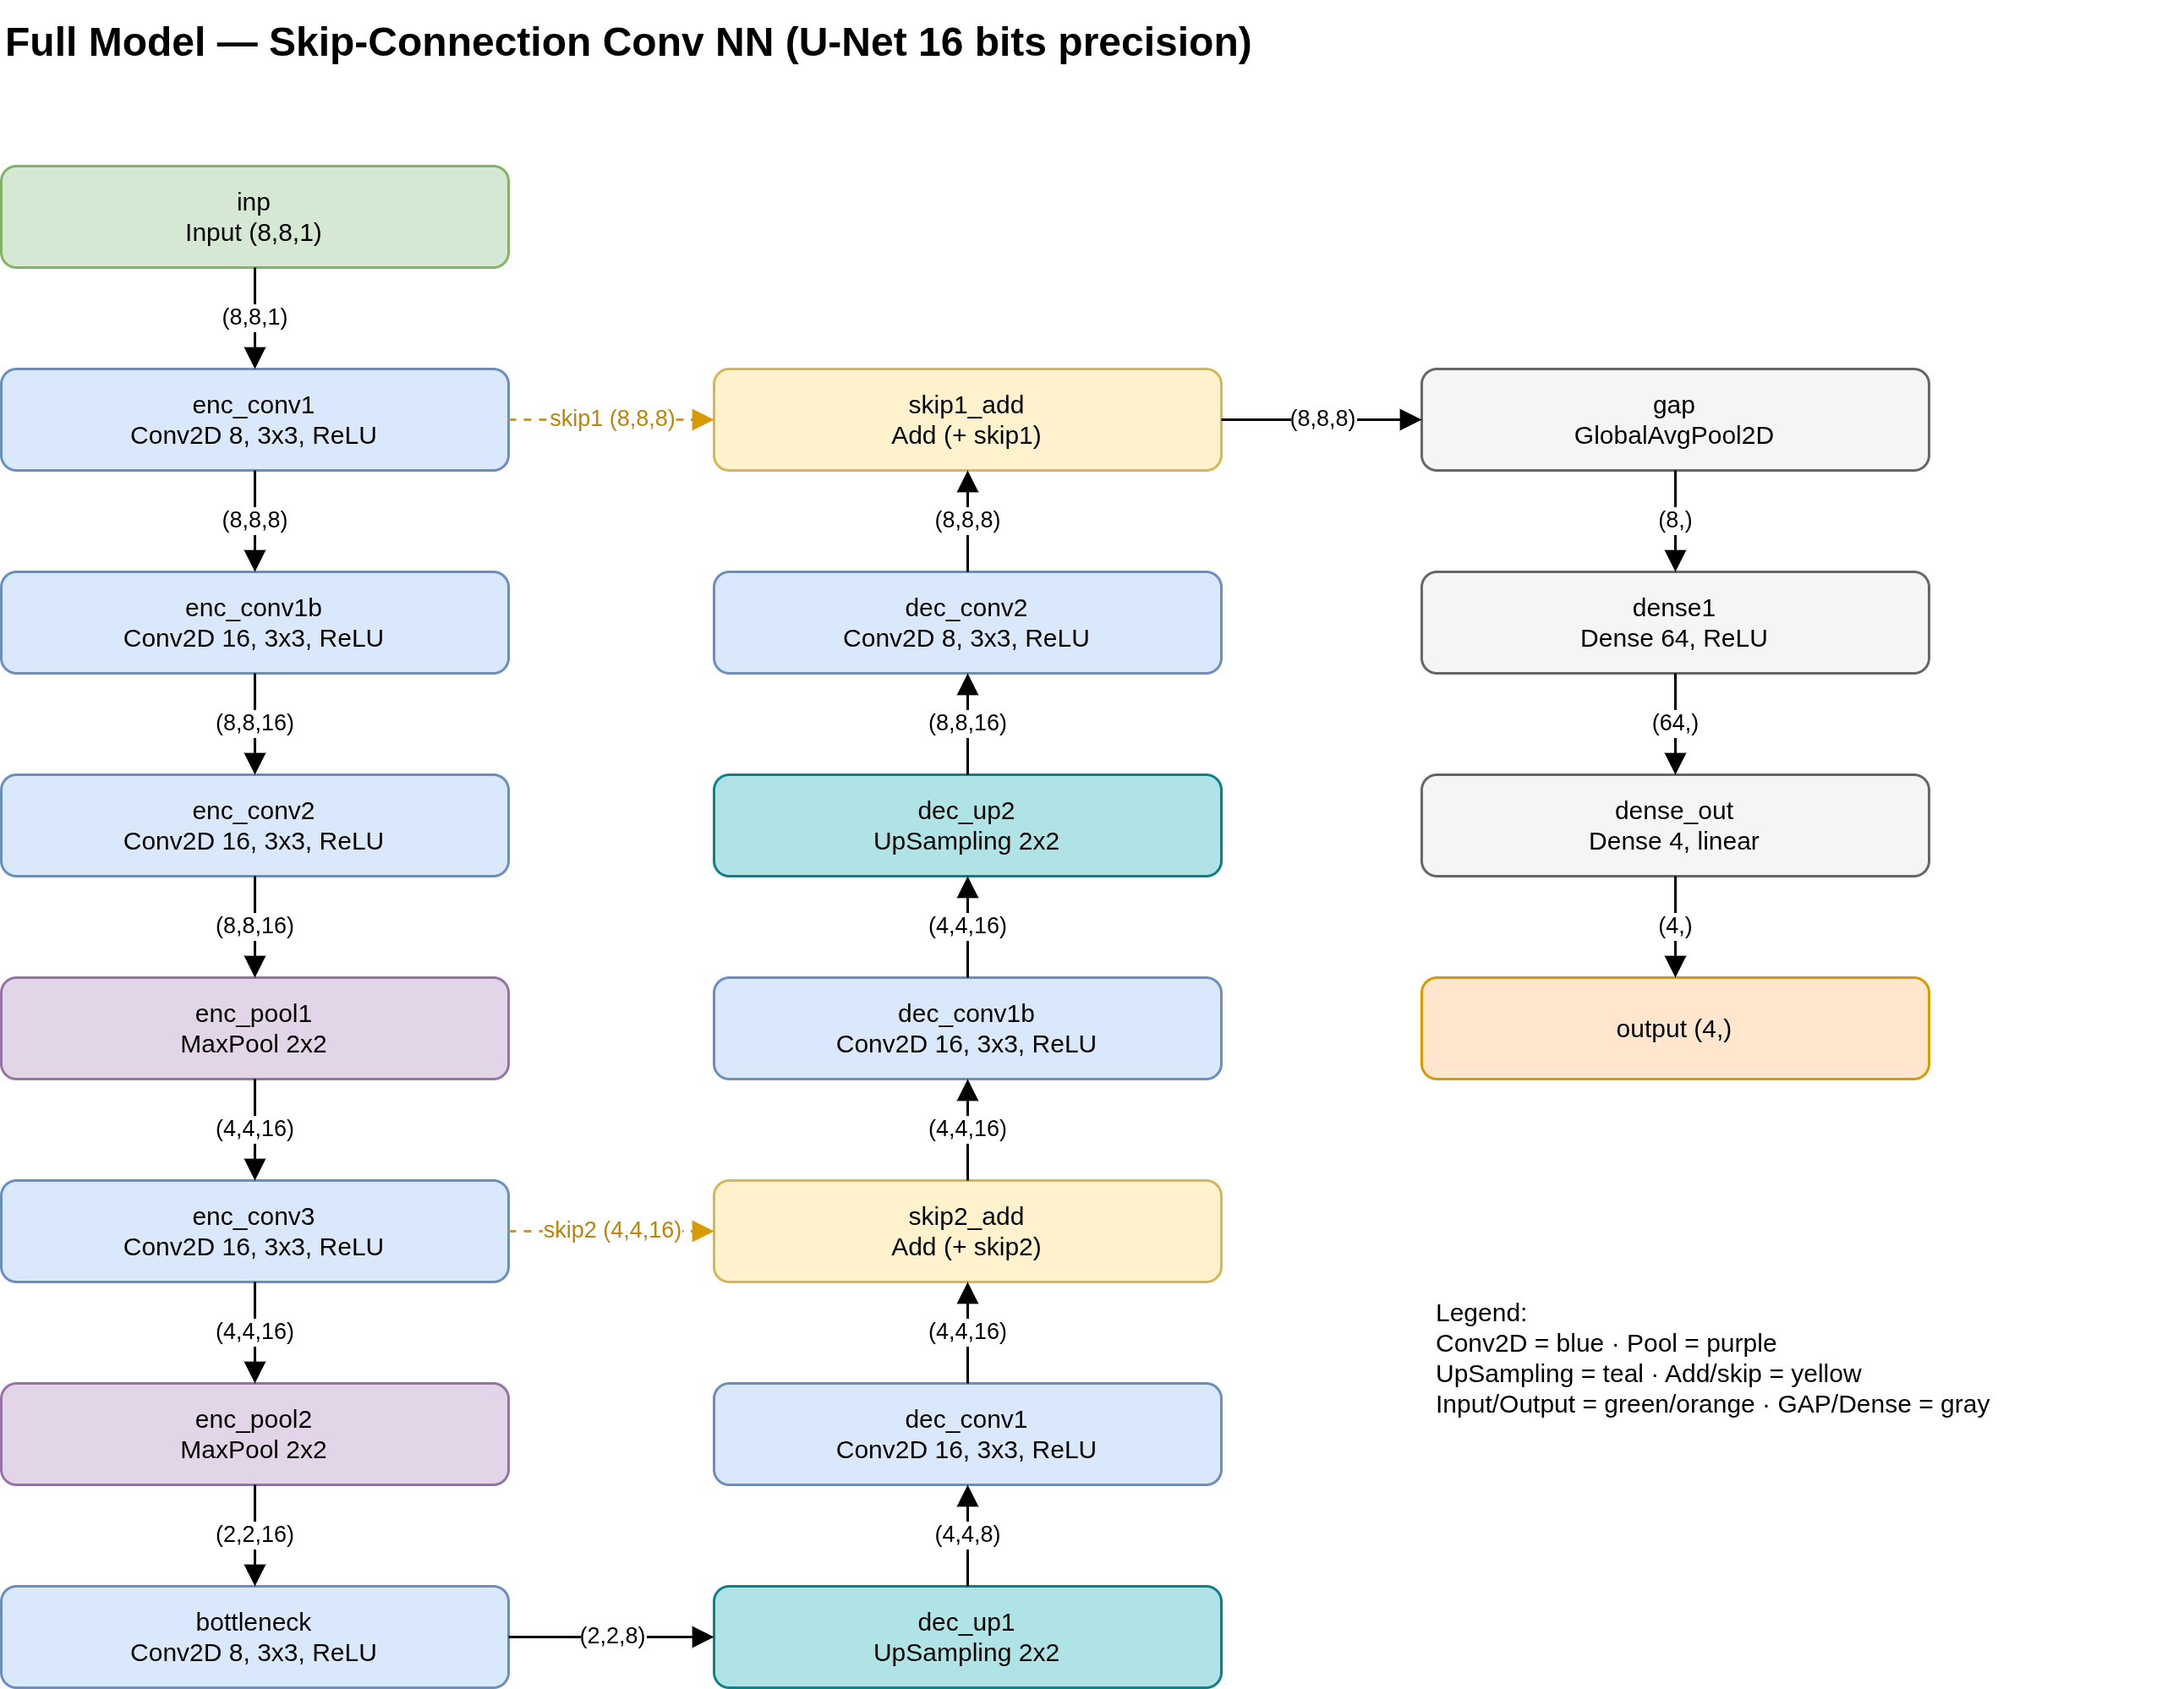
\includegraphics[width=\linewidth]{model_full.png}
  \caption{Skip-connection convolutional network (U-Net style) used for the experiment.}
  \label{fig:model_full}
\end{figure} 

The model takes an \texttt{(8,8,1)} input and produces a length-4 output vector. Every convolutional layer uses a $3\times3$ kernel with \texttt{same} padding and ReLU activation, so the spatial size changes only at the pooling and upsampling layers. The network is partitioned into four sequential parts, which map naturally onto the reconfigurable modules:

\begin{enumerate}
  \item \textbf{Encoder-A:} \texttt{enc\_conv1} (Conv2D~8) produces the first skip tensor \texttt{skip1} \texttt{(8,8,8)}; \texttt{enc\_conv1b} and \texttt{enc\_conv2} (Conv2D~16) refine the features, and \texttt{enc\_pool1} (MaxPool~$2\times2$) downsamples to \texttt{(4,4,16)}.
  \item \textbf{Encoder-B + Bottleneck:} \texttt{enc\_conv3} (Conv2D~16) produces the second skip tensor \texttt{skip2} \texttt{(4,4,16)}; \texttt{enc\_pool2} downsamples to \texttt{(2,2,16)}, and the \texttt{bottleneck} (Conv2D~8) compresses to \texttt{(2,2,8)}.
  \item \textbf{Decoder-A:} \texttt{dec\_up1} (UpSampling~$2\times2$) restores \texttt{(4,4,8)}; \texttt{dec\_conv1} (Conv2D~16) is fused with \texttt{skip2} by element-wise addition at \texttt{skip2\_add}, followed by \texttt{dec\_conv1b} (Conv2D~16) $\rightarrow$ \texttt{(4,4,16)}.
  \item \textbf{Decoder-B + Head:} \texttt{dec\_up2} restores \texttt{(8,8,16)}; \texttt{dec\_conv2} (Conv2D~8) is fused with \texttt{skip1} by element-wise addition at \texttt{skip1\_add} \texttt{(8,8,8)}. The classification head then applies \texttt{gap} (GlobalAveragePooling2D), \texttt{dense1} (Dense~64, ReLU), and \texttt{dense\_out} (Dense~4, linear) to yield the final \texttt{(4,)} output.
\end{enumerate}

Note that the two skip connections fuse features by \emph{addition} rather than concatenation, so the channel counts of the encoder and decoder tensors must match at each fusion point. The model is trained with the Adam optimizer and a categorical cross-entropy loss.


\subsection{Model Partitioning}

We set up two use-case scenarios: first, we divide the model into four parts, and second, we divide it into two parts.

\subsubsection{Four-Part Partitioning}

In the four-part scheme, the model is split at the boundaries of the four sequential parts and mapped onto two physical reconfigurable regions over four reconfiguration phases, as shown in Figure~\ref{fig:model_4sub}. The blue parts (1 and 3) are loaded into \emph{region~0}, and the orange parts (2 and 4) into \emph{region~1}; the two regions are reconfigured alternately, so that one region can execute its current part while the other is being reconfigured for the next. 

\begin{figure}[H]
  \centering
  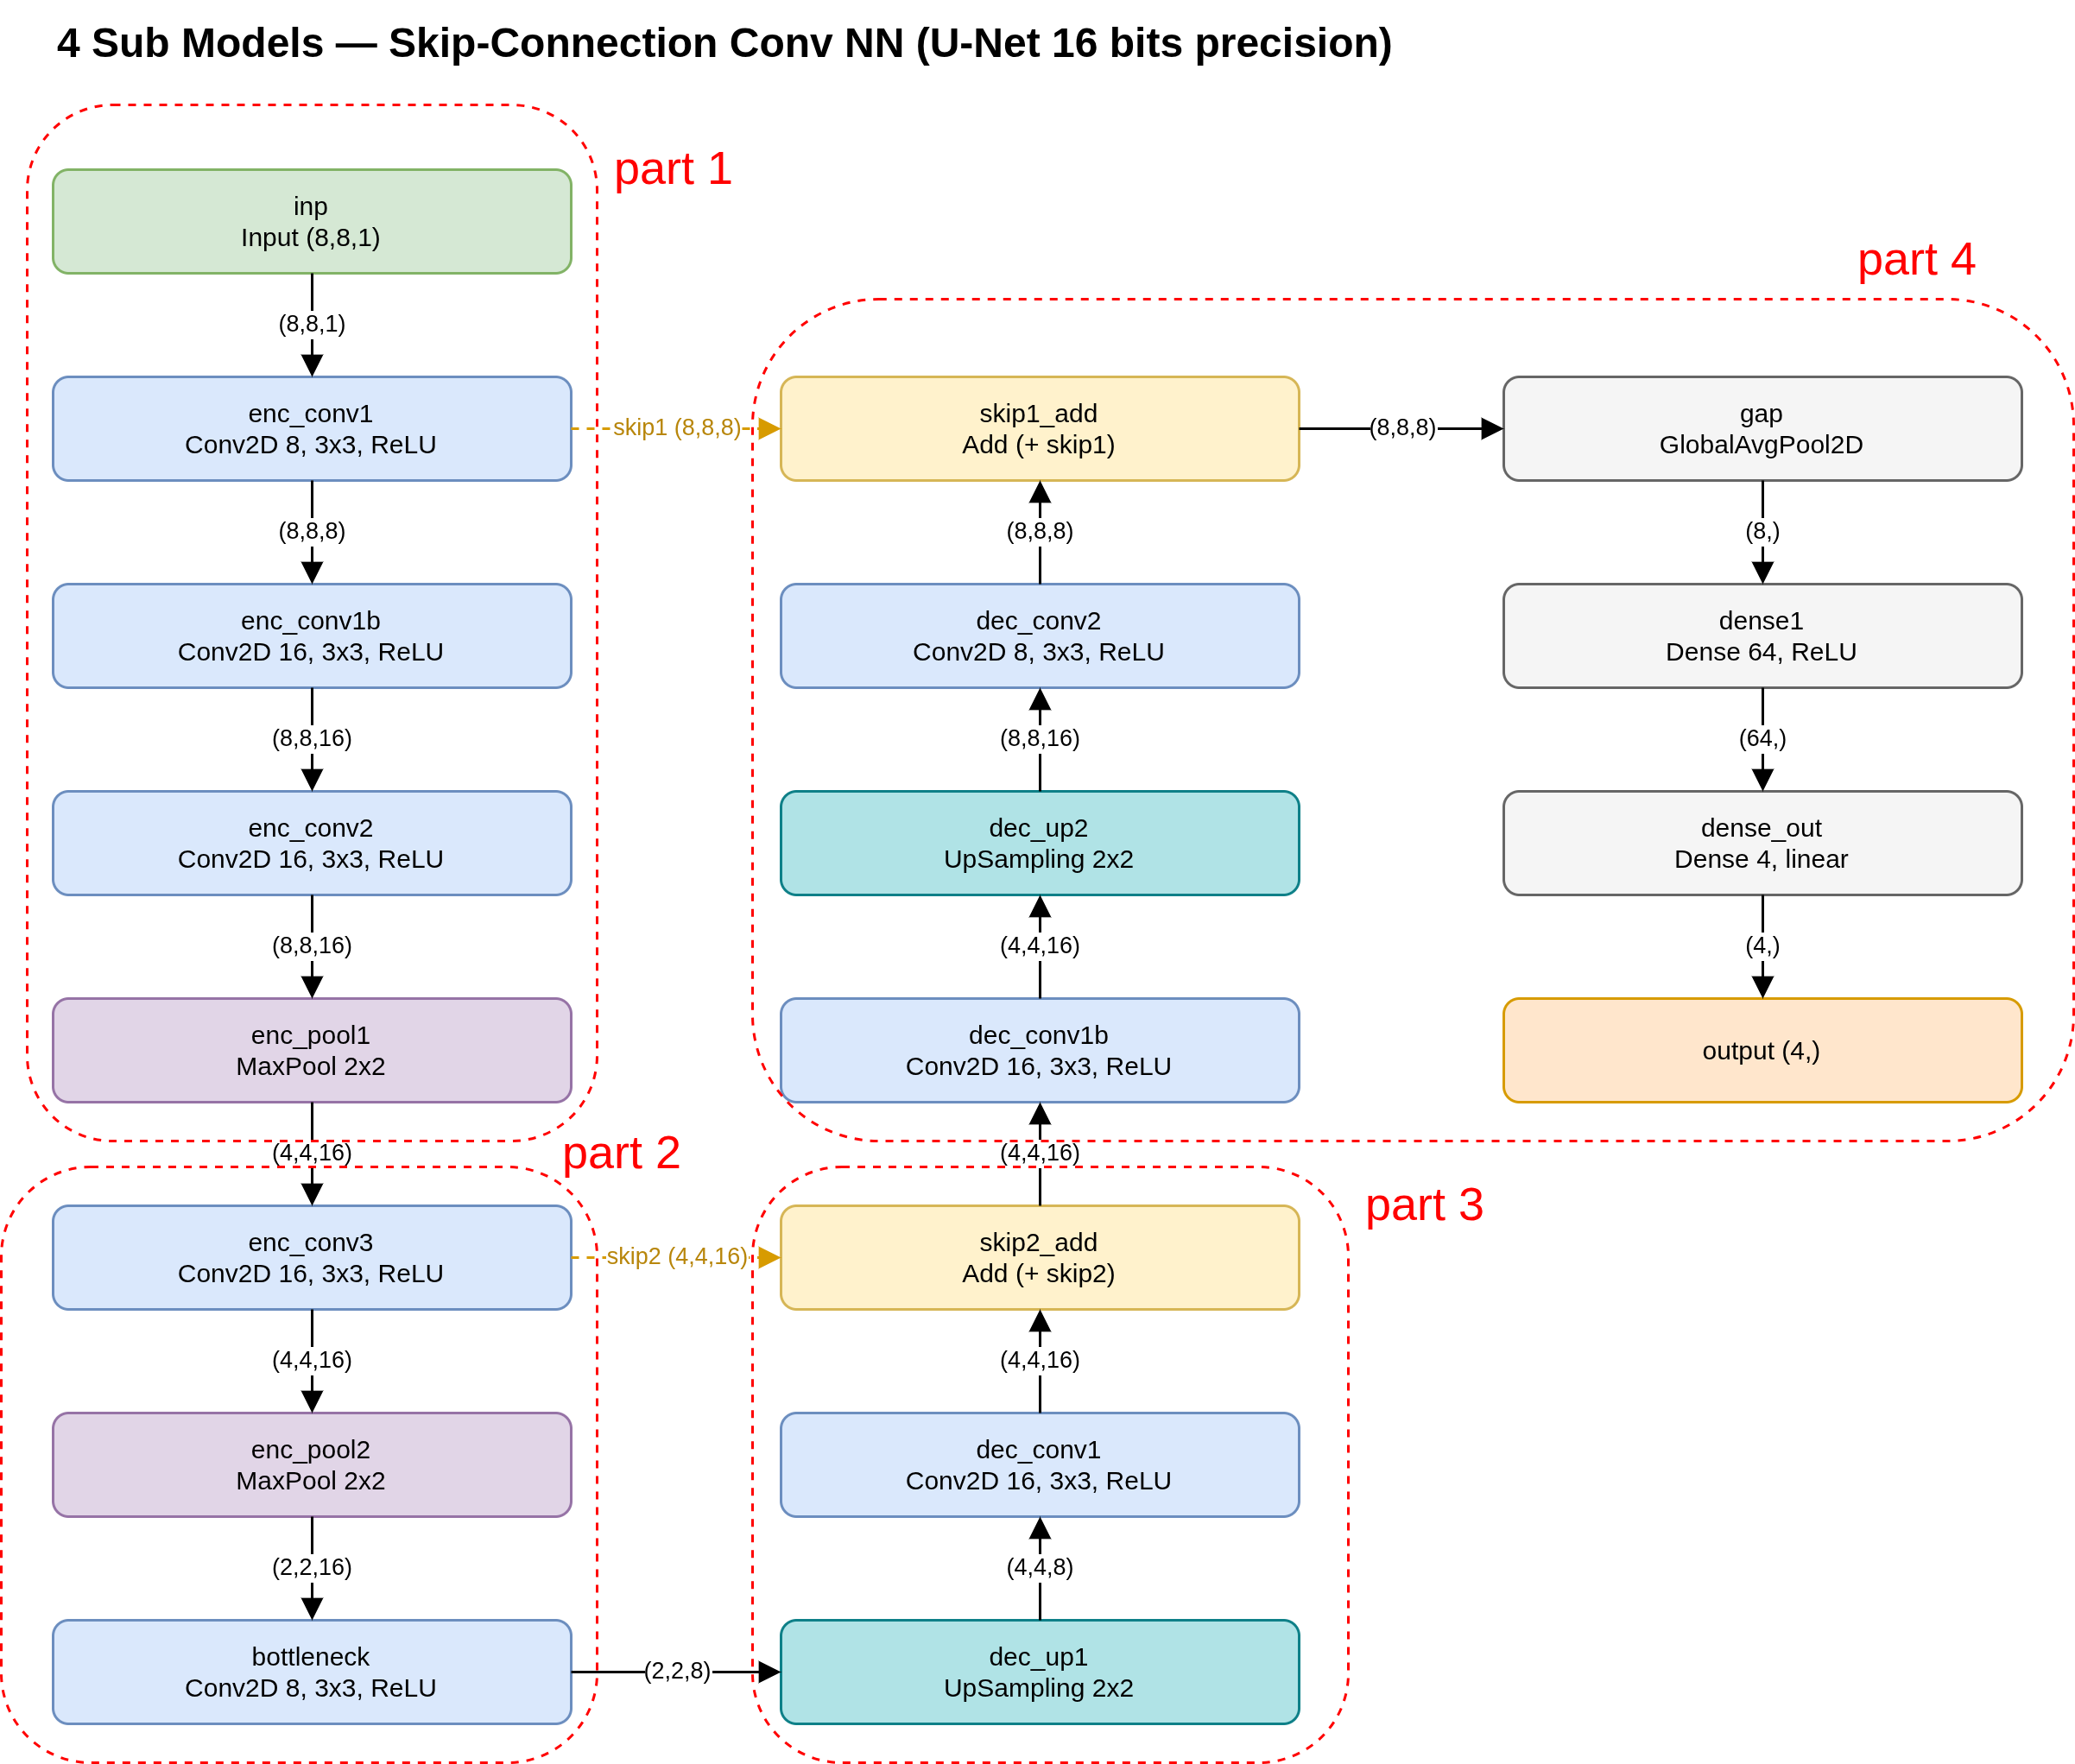
\includegraphics[width=\linewidth]{4-sub-model.drawio.png}
  \caption{Four-part partitioning scheme: colored boxes are the DFX regions/phases, solid purple arrows are the main inter-partition streams, and dashed gold arrows are the skip streams.}
  \label{fig:model_4sub}
\end{figure}

The four parts map to the physical regions and reconfiguration phases as shown in Table~\ref{tab:four_part_map}.

\begin{table}[H]
  \centering
  \caption{Mapping of the four model parts to physical regions and reconfiguration phases.}
  \label{tab:four_part_map}
  \begin{tabular}{cl cc}
    \toprule
    Part & Stage & Region & Phase \\
    \midrule
    1 & Encoder-A             & 0 & 0 \\
    2 & Encoder-B + Bottleneck & 1 & 1 \\
    3 & Decoder-A             & 0 & 2 \\
    4 & Decoder-B + Head      & 1 & 3 \\
    \bottomrule
  \end{tabular} 
\end{table}

Region~0 hosts Parts~1 and~3 while region~1 hosts Parts~2 and~4, so each region is reused twice across the pipeline.

\subsubsection{Two-Part Partitioning}

In the two-part scheme, the model is split at the bottleneck into two halves, as shown in Figure~\ref{fig:model_2sub}. Half~A holds the entire encoder and bottleneck (Parts~1--2), while Half~B holds the decoder and classification head (Parts~3--4). Since the split is a single boundary, the main bottleneck stream and both skip streams all cross from Half~A to Half~B.

\begin{figure}[H]
  \centering
  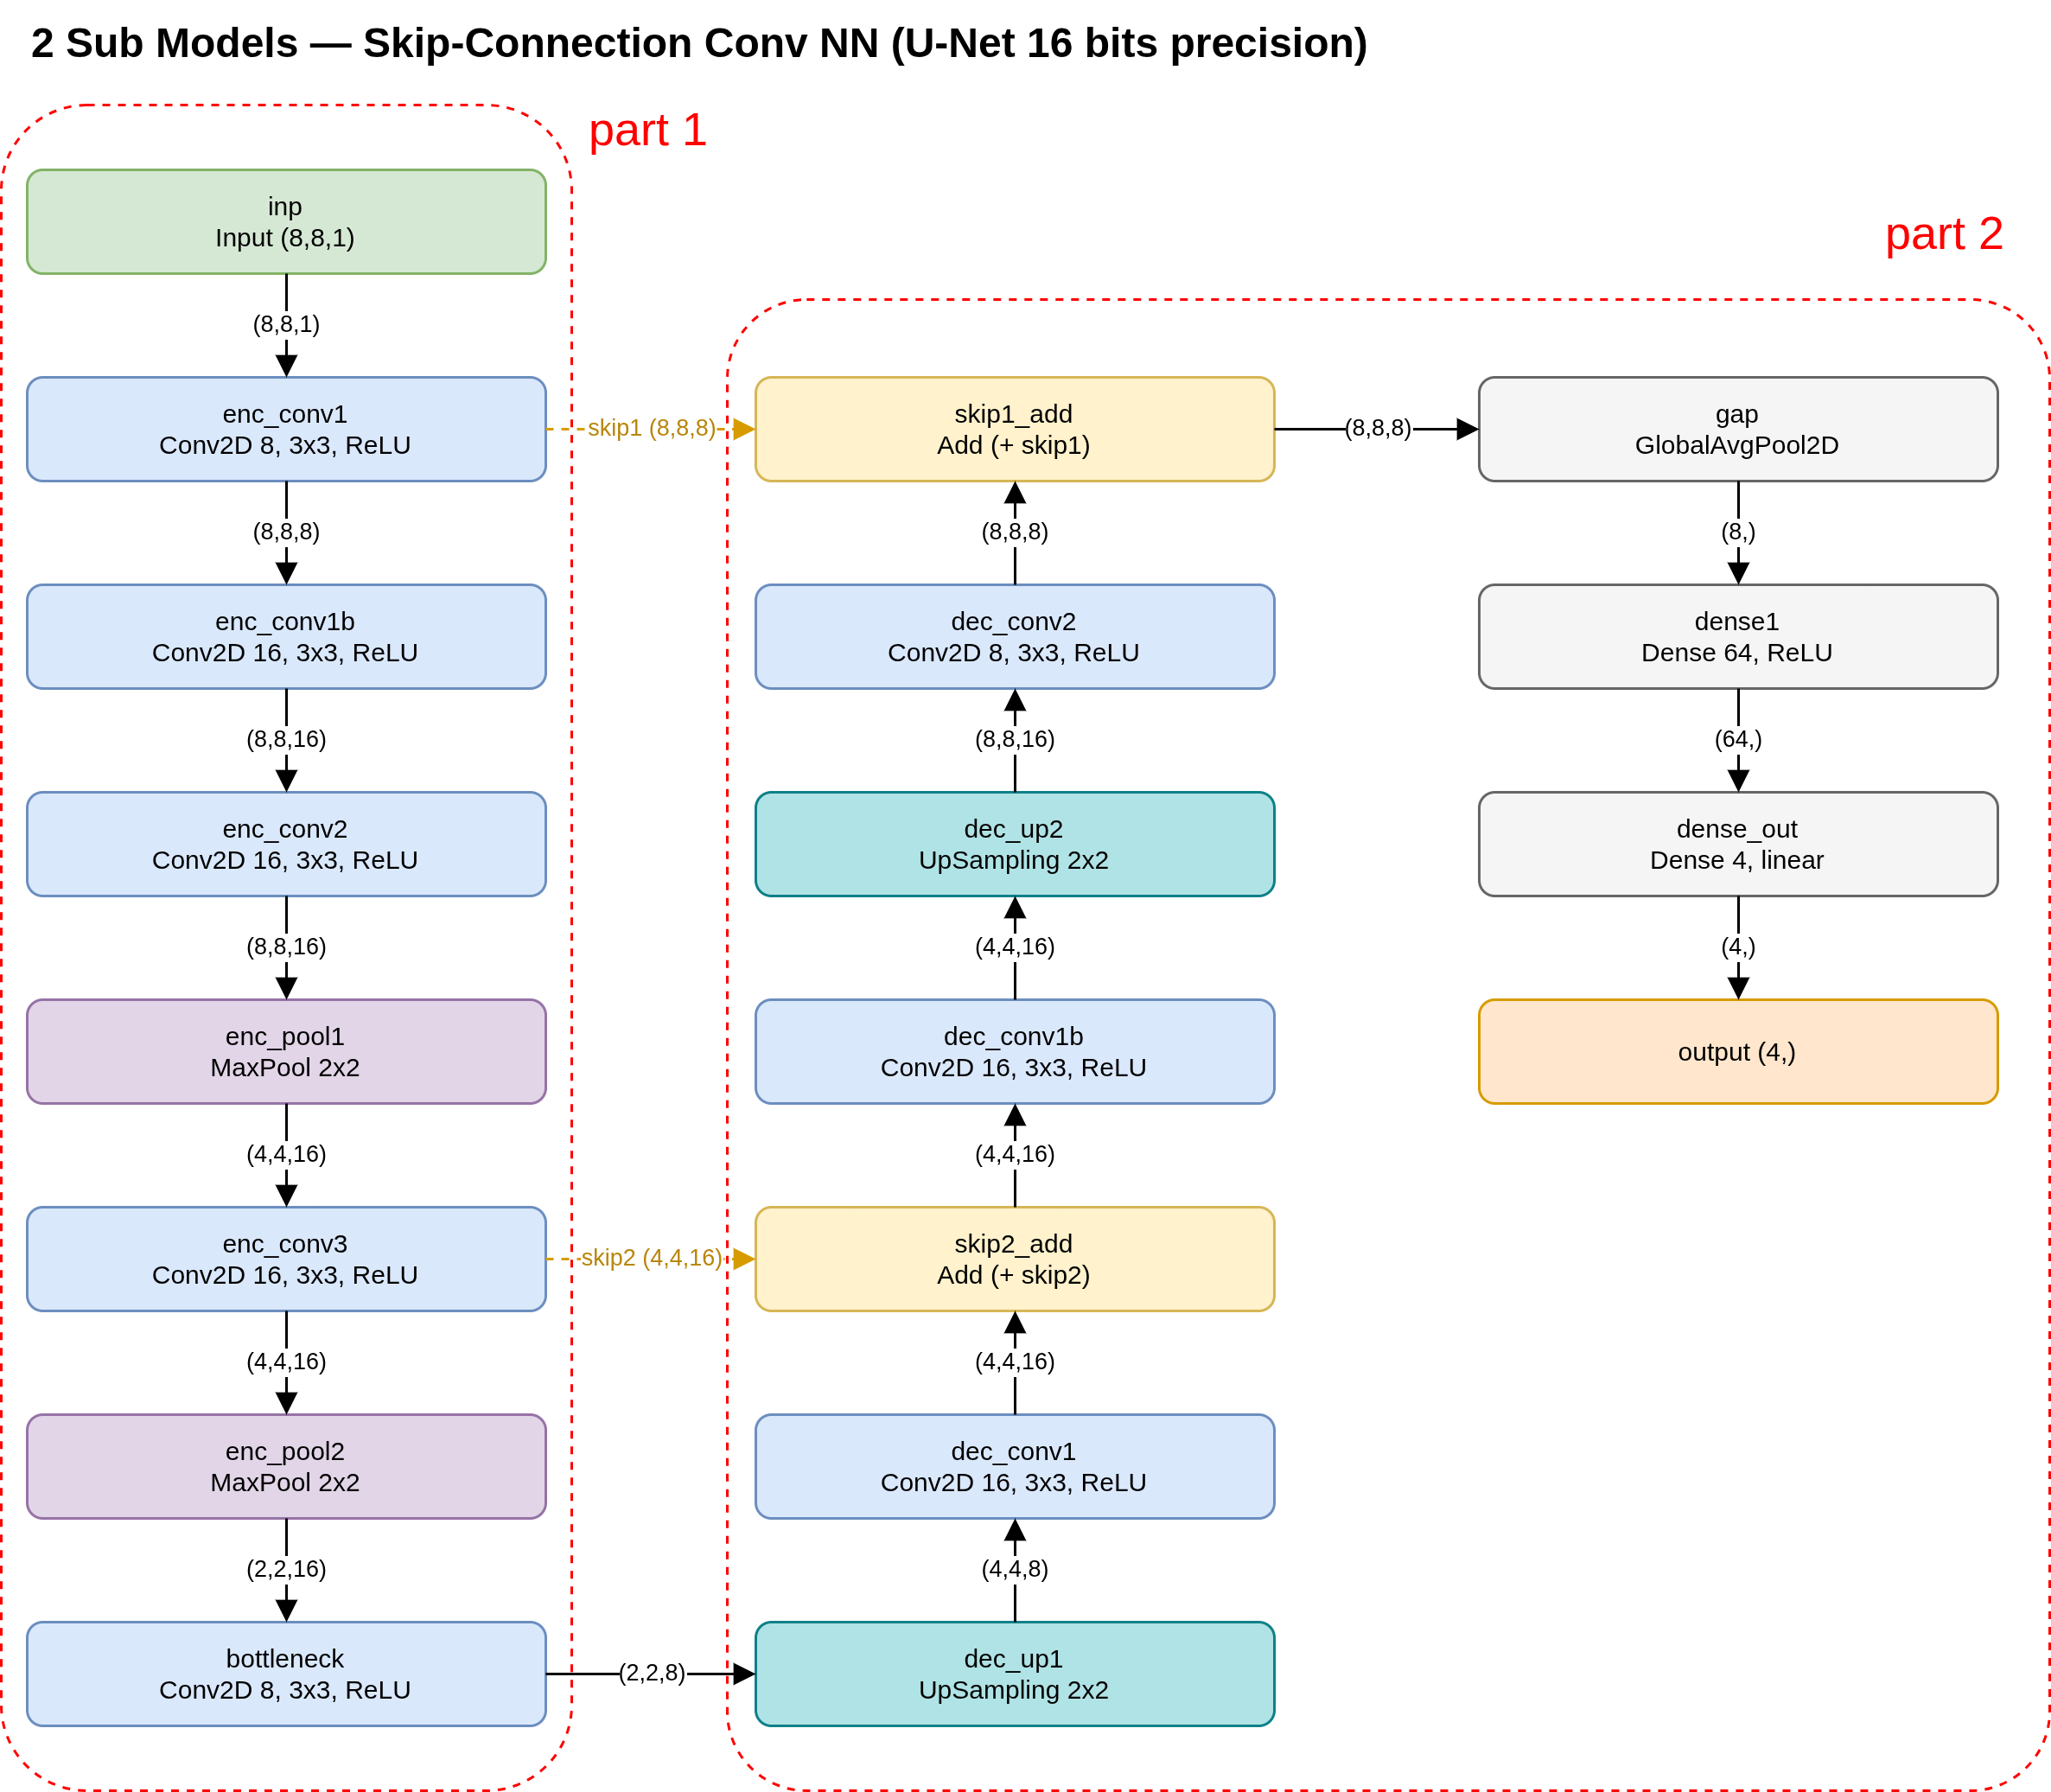
\includegraphics[width=\linewidth]{2-sub-model.png}
  \caption{Two-part partitioning scheme: the model is split at the bottleneck into Half~A (encoder + bottleneck) and Half~B (decoder + head).}
  \label{fig:model_2sub}
\end{figure}

The two halves map to the physical regions and reconfiguration phases as shown in Table~\ref{tab:two_part_map}.

\begin{table}[H]
  \centering
  \caption{Mapping of the two model halves to physical regions and reconfiguration phases.}
  \label{tab:two_part_map}
  \begin{tabular}{cl cc}
    \toprule
    Half & Stage & Region & Phase \\
    \midrule
    A & Encoder + Bottleneck & 0 & 0 \\
    B & Decoder + Head       & 0 & 1 \\
    \bottomrule
  \end{tabular}
\end{table}


\subsection{DFX Streamer Management for current experiments}

\subsubsection{DFX Streamer allocation algorithm}

\begin{figure}[H]
  \centering
  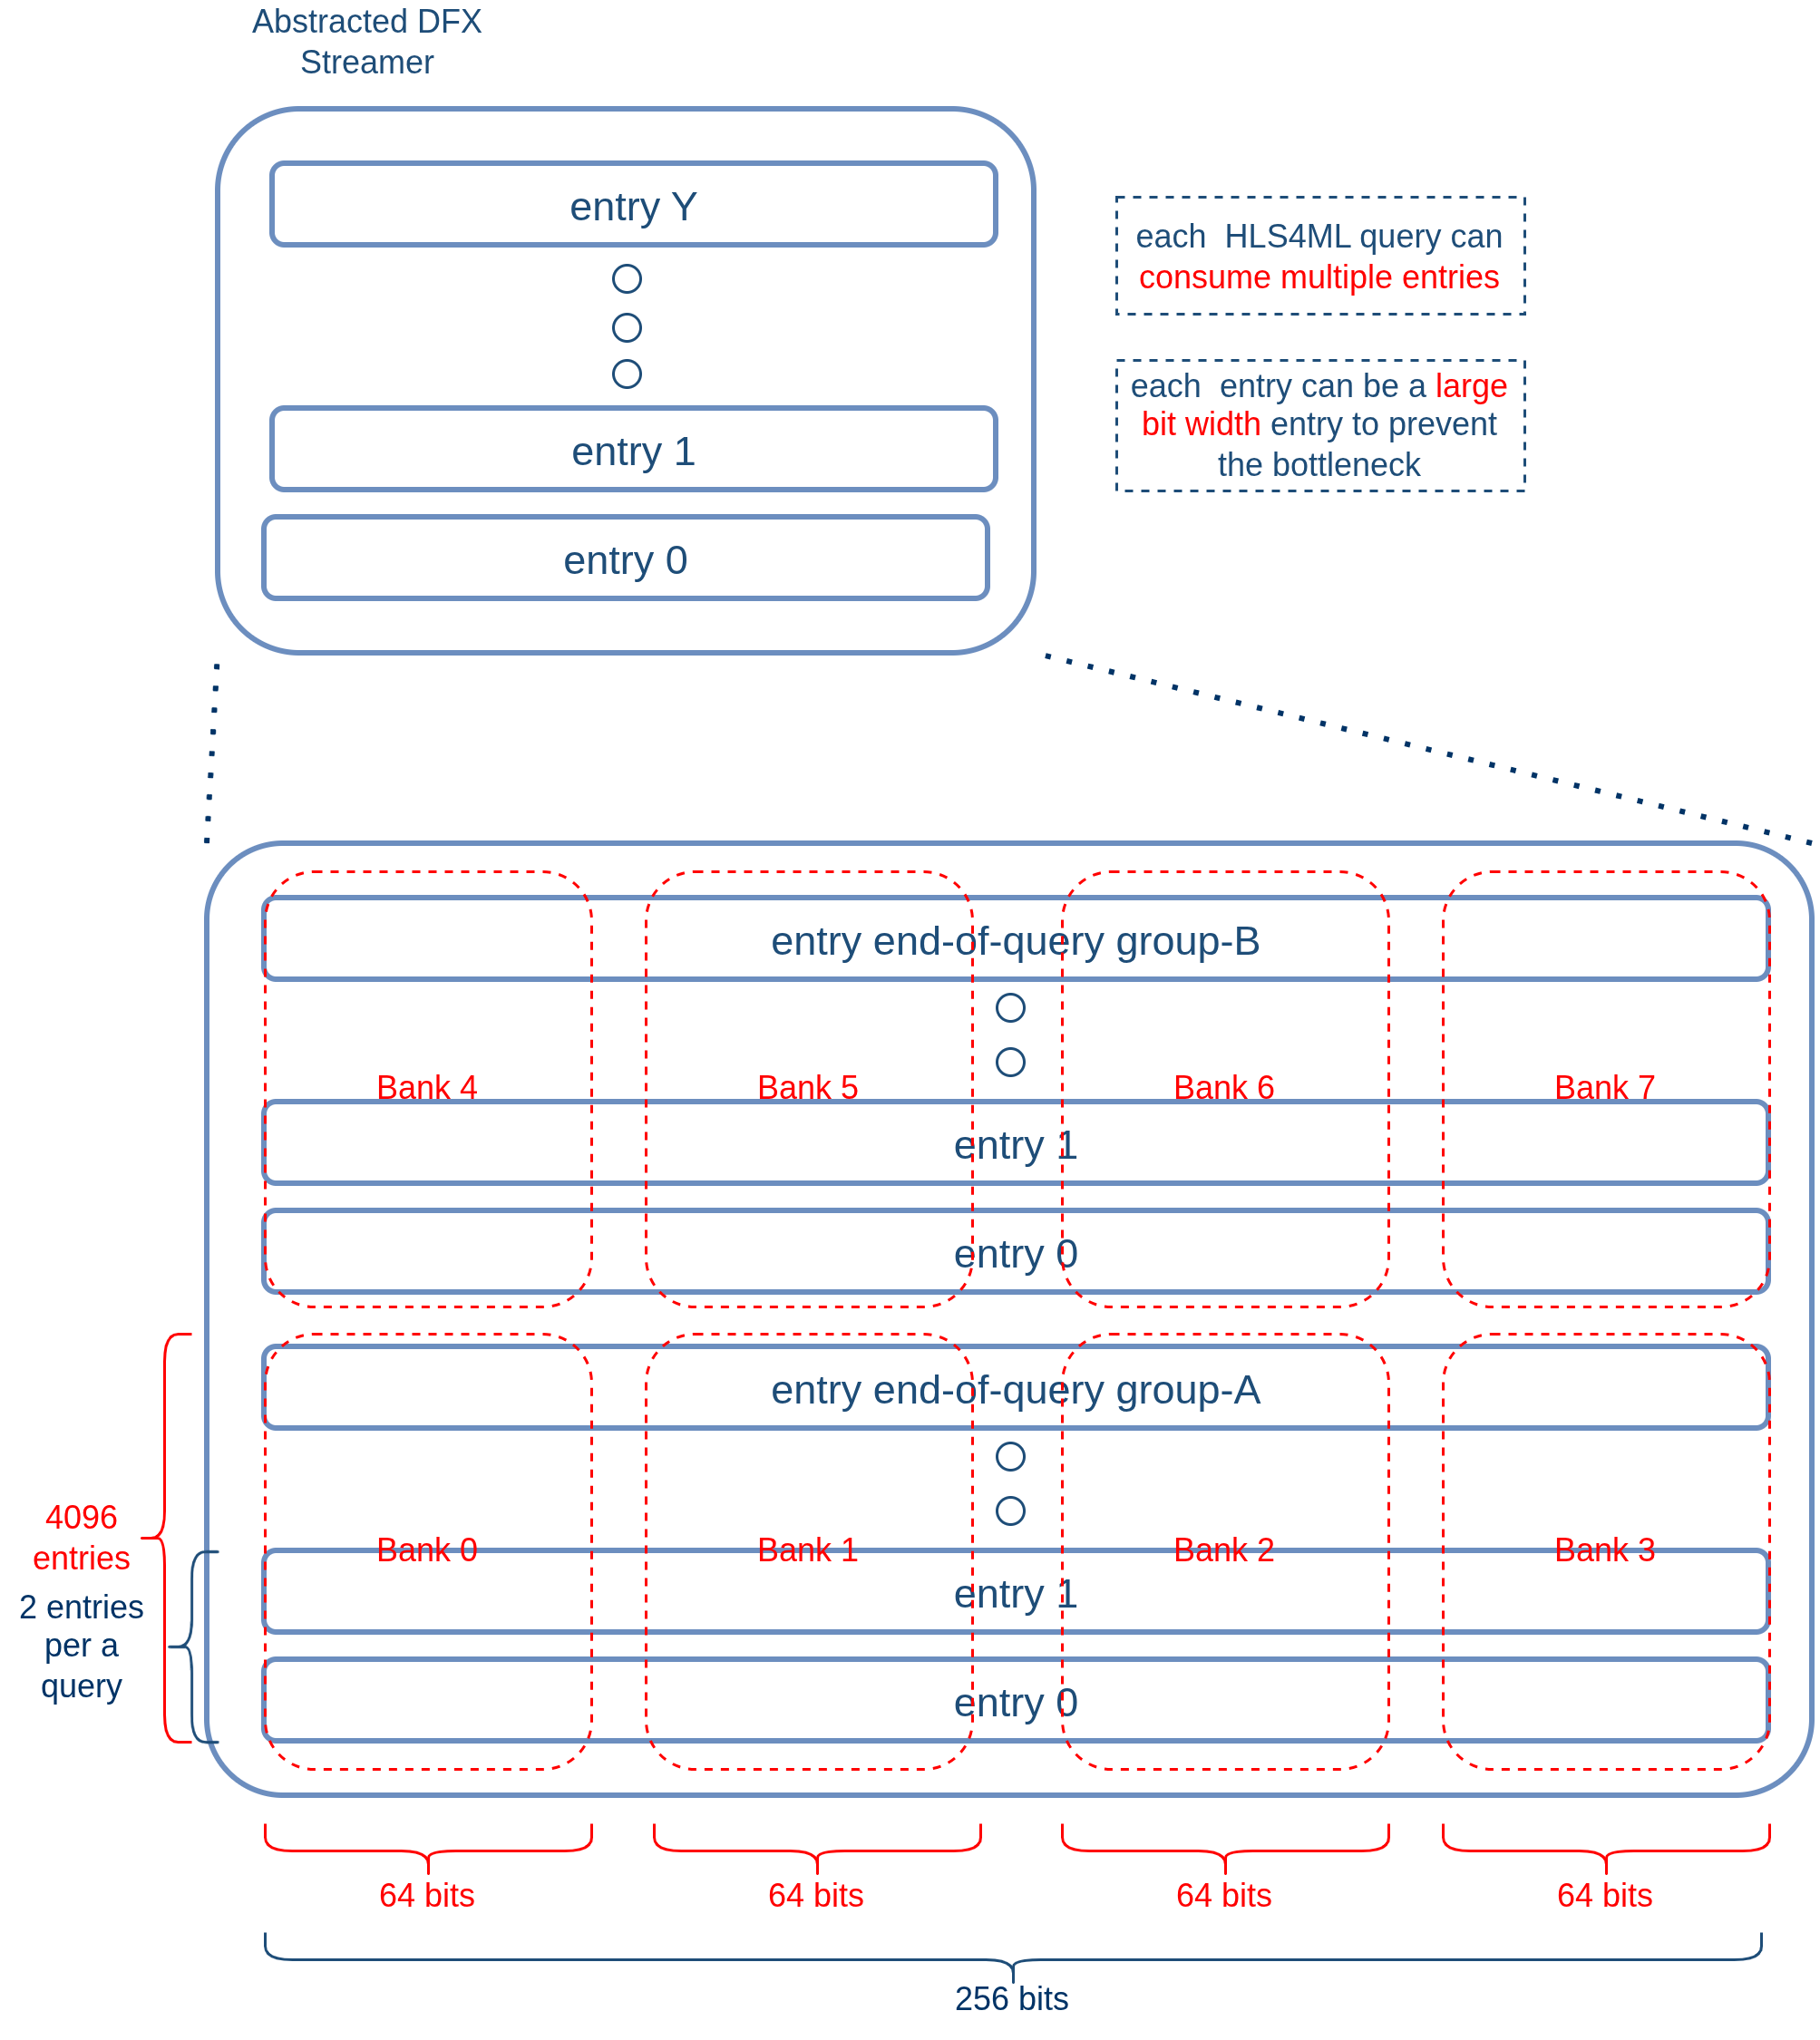
\includegraphics[height=0.6\textheight]{magic_streamer_algo.png}
  \caption{DFX (magic) streamer buffer allocation visualization.}
  \label{fig:magic_streamer_vis}
\end{figure}

 
Imagin the dfx streamer as an the fifo consisted of multiple entries (\ref{fig:magic_streamer_vis}). the entry is supposed to hold the data out from the HLS4ML layer stream. For instance, if the HLS4ML stream dump (2,1,16) with 16 bits precision for each query. Therefore, the HLS4ML will dump 16 x 16 = 256 bits output for each cycle.

Assume that Xilinx's URAM provides 64 bits per bank; in that case, we may need at least 4 banks at the output. And the URAM can support 4096 rows therefore we can hold 4096/(2*1) = 2048 for this set. User can have more of set the URAM to support more queries.




The overall buffer-sizing procedure is summarised in Algorithm~\ref{alg:magic_streamer}. It works in four stages:

\begin{enumerate}
  \item compute the bank geometry of every stream;
  \item hand each stream a physical streamer for the phases it is alive, reusing a free streamer of the same size and region whenever possible;
  \item spend the remaining bank budget on the streamer with the smallest capacity;
  \item report the result.
\end{enumerate}

\begin{algorithm}[H] 
\caption{DFX streamer buffer allocation}
\label{alg:magic_streamer}
\begin{algorithmic}[1]
\Require streams (each with \emph{shape}, \emph{precision}, \emph{region}, \emph{allocPhase}, \emph{freePhase}); bank budget $N$; phase count $P$; bank width $BW$ and depth $BD$
\Ensure for every streamer: its bank count and buffered-query capacity
\Statex
\State \textbf{Stage 1: per-stream geometry}
\For{each stream $s$}
    \State $entries \gets$ product of all but the last dimension of $s.shape$ \Comment{items per query}
    \State $bits \gets s.precision \times (\text{last dimension of } s.shape)$
    \State $s.banks \gets \lceil bits / BW \rceil$ \Comment{banks needed for one item}
    \State $s.cap \gets \lfloor BD / entries \rfloor$ \Comment{queries one bank set can hold}
    \If{$s.cap = 0$}
        \State \textbf{error}: ``one query does not fit in a bank set''
    \EndIf
\EndFor
\Statex
\State \textbf{Stage 2: allocate streamers across phases (reuse when possible)}
\State $free \gets \emptyset$;\quad $using \gets \emptyset$;\quad $streamers \gets \emptyset$
\For{$phase \gets 0$ \textbf{to} $P-1$}
    \ForAll{stream $s$ with $s.allocPhase = phase$}
        \State look for a free streamer $f$ with $f.banks = s.banks$ \textbf{and} $f.region = s.region$
        \If{such $f$ exists}
            \State attach $s$ to $f$;\quad $f.freePhase \gets s.freePhase$;\quad move $f$ from $free$ to $using$
        \Else
            \State create new streamer ($banks = s.banks$, $region = s.region$, $mul = 1$, holding $s$)
            \State add it to $using$ and to $streamers$
        \EndIf
    \EndFor
    \State move each $using$ streamer whose $freePhase = phase$ back to $free$ \Comment{data no longer needed}
\EndFor
\If{$streamers = \emptyset$}
    \State \Return $\{streamers,\ banksUsed = 0\}$
\EndIf
\Statex
\State \textbf{Stage 3: grow buffers within the bank budget (water-filling)}
\While{\textbf{true}}
    \State $banksUsed \gets \sum_{d \in streamers} d.banks \times d.mul$
    \State $b \gets$ streamer with the smallest capacity $d.mul \times d.cap$ \Comment{the bottleneck}
    \If{$banksUsed + b.banks > N$}
        \State \textbf{break} \Comment{next growth would exceed the budget}
    \EndIf
    \State $b.mul \gets b.mul + 1$ \Comment{give the bottleneck one more bank set}
\EndWhile
\Statex
\State \textbf{Stage 4: report}
\State \Return $\{streamers,\ banksUsed,\ \min_{d \in streamers}(d.mul \times d.cap)\}$
\end{algorithmic}
\end{algorithm}


\subsubsection{4-sub model DFX streamer allocation}

Running the allocation algorithm on the four-part scheme yields the streamer schedule shown in Figure~\ref{fig:4_part_mgs_schedule}.

\begin{figure}[H]
  \centering
  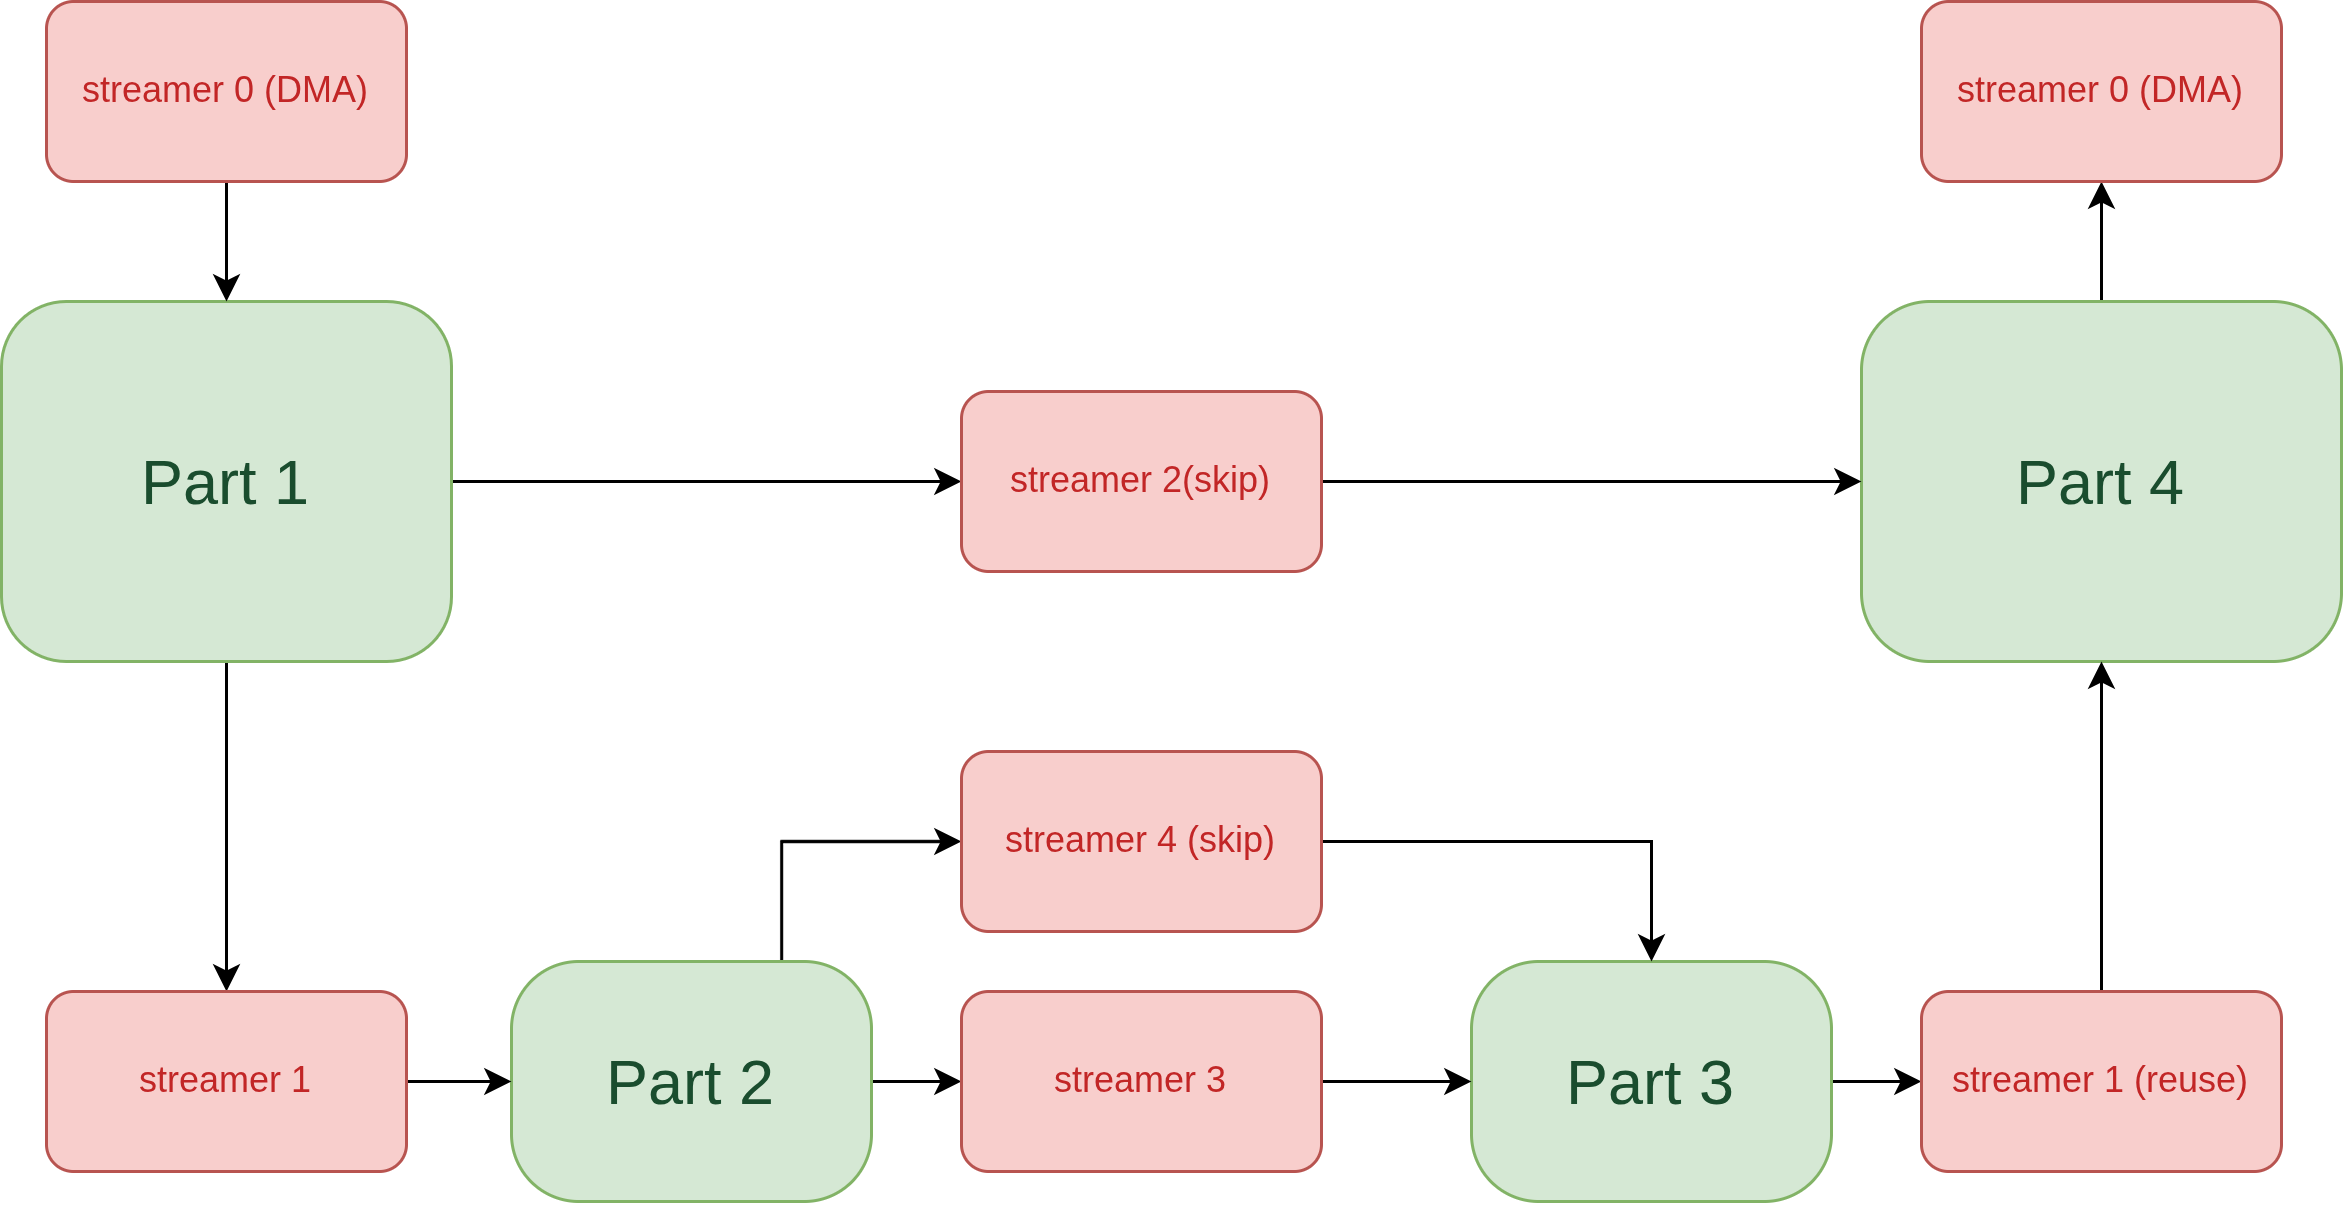
\includegraphics[width=0.7\linewidth]{4_part_mgs_schedule.png}
  \caption{DFX streamer schedule for the four-part partitioning scheme.}
  \label{fig:4_part_mgs_schedule}
\end{figure}

The resulting bank usage is summarised in Table~\ref{tab:four_part_alloc}. Four physical streamers are created: \texttt{streamer\_1} is reused by both region-0 main streams (\texttt{p0\_main} then \texttt{p2\_main}), while the long-lived \texttt{p0\_skip} gets its own streamer with the largest number of bank sets. The total banks used, $\sum (\text{banks/set} \times \text{amt set}) = 64$, stays within the bank budget $N = 64$.

\begin{table}[H]
  \centering
  \footnotesize
  \setlength{\tabcolsep}{4pt}
  \caption{DFX streamer bank usage for the four-part scheme.}
  \label{tab:four_part_alloc}
  \begin{tabular}{l c c c c c}
    \toprule
    Streamer & Region & banks/set & Free phase & amt set & banks (banks/set $\times$ amt set) \\
    \midrule
    streamer\_1 & 0 & 4 & 3 &  4 & 16 \\
    streamer\_2 & 0 & 2 & 3 & 15 & 30 \\
    streamer\_3 & 1 & 2 & 2 &  1 &  2 \\
    streamer\_4 & 1 & 4 & 2 &  4 & 16 \\
    \midrule
    \multicolumn{5}{r}{Total banks used} & 64 \\
    \bottomrule
  \end{tabular} 
\end{table}

The columns of Table~\ref{tab:four_part_alloc} are defined in Table~\ref{tab:alloc_cols}.

\begin{table}[H]
  \centering
  \footnotesize
  \caption{Column definitions for Table~\ref{tab:four_part_alloc}.}
  \label{tab:alloc_cols}
  \begin{tabular}{l l p{7.5cm}}
    \toprule
    Column & Code variable & Meaning \\
    \midrule
    Streamer   & \texttt{name}                  & Identifier of the physical DFX streamer (a URAM bank group). \\
    Region     & \texttt{region}                & Reconfigurable region whose data this streamer holds. \\
    banks/set  & \texttt{amt\_banks\_per\_entry} & URAM banks in one bank set (banks needed to store one entry). \\
    Free phase & \texttt{next\_fin\_phase}      & Phase at which the stored data is consumed, after which the streamer may be reused. \\
    amt set    & \texttt{mul\_factor}           & Number of bank sets replicated for this streamer. \\
    banks      & ---                            & Total banks used by this streamer, banks/set $\times$ amt set. \\
    \bottomrule 
  \end{tabular}
\end{table}

Table~\ref{tab:four_part_streams} lists each inter-partition stream, the streamer it is assigned to, the entries it produces per query (\texttt{amt\_entry\_per\_query}), the queries one bank set can hold (\texttt{amt\_query\_per\_bankGrp}), and the resulting buffered-query capacity (\texttt{total\_query} $=$ amt set $\times$ queries/set). \texttt{p0\_skip} reaches only 960 (red), making it the bottleneck on the overall buffered-query count.

\begin{table}[H]
  \centering
  \footnotesize
  \caption{Per-stream buffering capacity for the four-part scheme.}
  \label{tab:four_part_streams}
  \begin{tabular}{l l c c c}
    \toprule
    Stream & Streamer & Entries/query & Queries/set & Total Q \\
    \midrule
    p0\_main & streamer\_1 & 16 &  256 & 1024 \\
    p2\_main & streamer\_1 & 16 &  256 & 1024 \\
    p0\_skip & streamer\_2 & 64 &   64 & \textcolor{red}{960} \\
    p1\_main & streamer\_3 &  4 & 1024 & 1024 \\
    p1\_skip & streamer\_4 & 16 &  256 & 1024 \\
    \bottomrule
  \end{tabular} 
\end{table}


\subsubsection{2-sub model DFX streamer allocation}

Running the allocation algorithm on the two-part scheme yields the streamer schedule shown in Figure~\ref{fig:2_part_mgs_schedule}.

\begin{figure}[H]
  \centering
  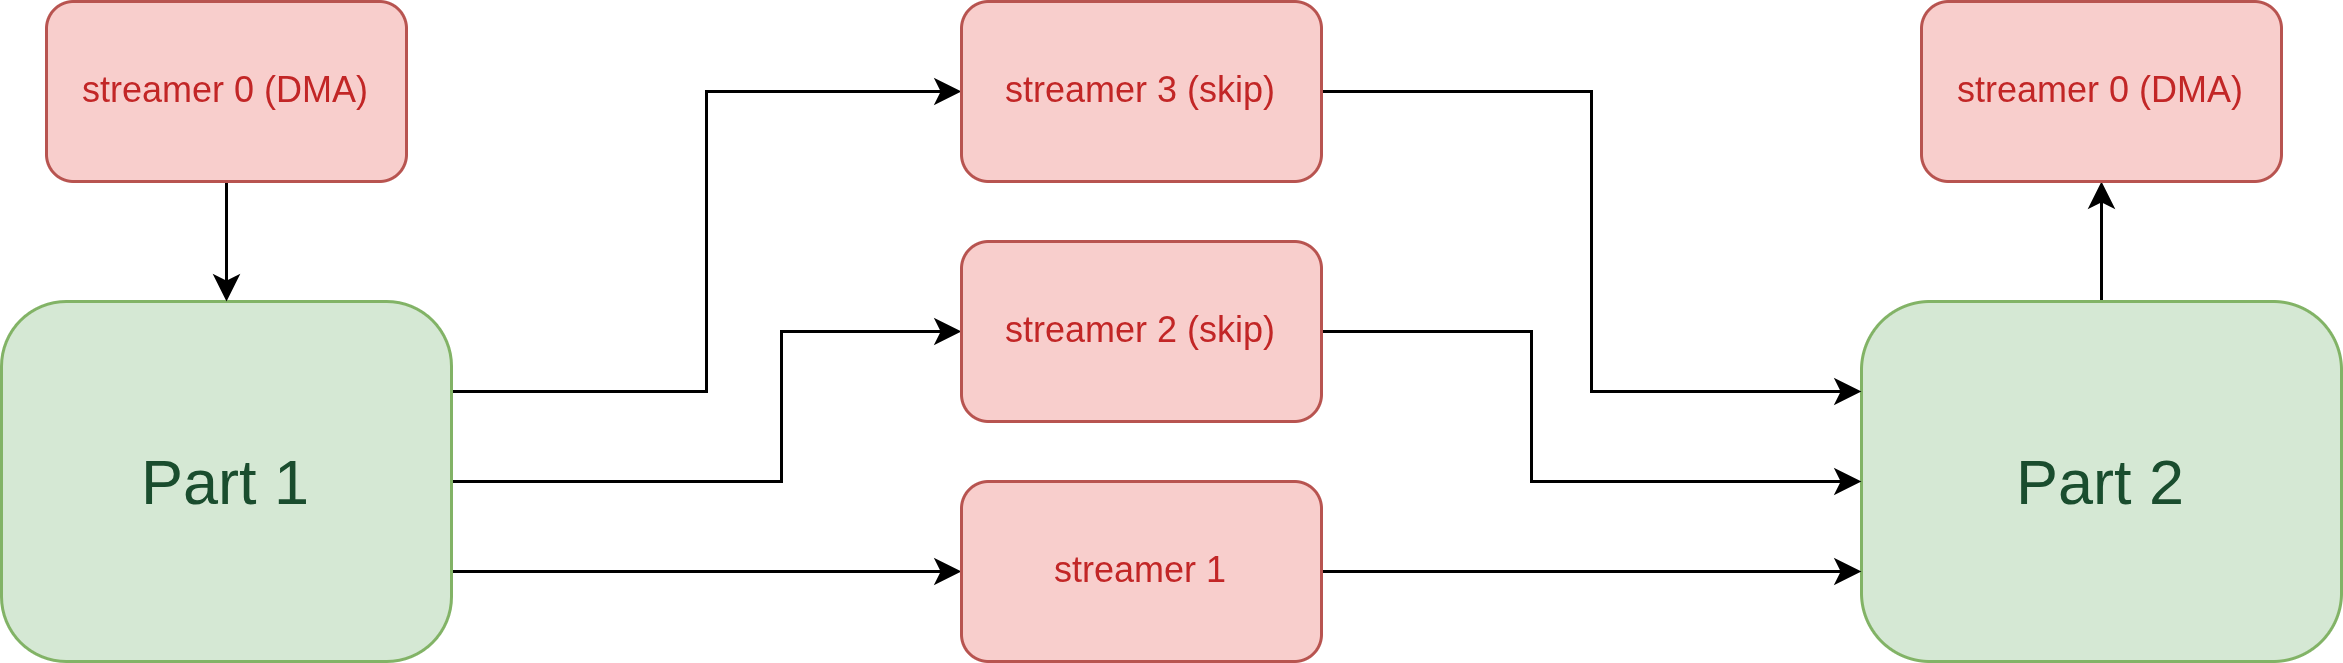
\includegraphics[width=0.7\linewidth]{2_part_mgs_schedule.png}
  \caption{DFX streamer schedule for the two-part partitioning scheme.}
  \label{fig:2_part_mgs_schedule}
\end{figure}

The resulting bank usage is summarised in Table~\ref{tab:two_part_alloc}. Because the model is split at a single boundary, the three crossing streams (\texttt{ha\_bneck}, \texttt{ha\_skip2}, \texttt{ha\_skip1}) are all alive at the same time, so each is given its own physical streamer and no reuse is possible. All three live in region~0 and are freed at phase~1, once Half~B has consumed them. The total banks used, $\sum (\text{banks/set} \times \text{amt set}) = 64$, exactly fills the bank budget $N = 64$. The columns have the same meaning as in Table~\ref{tab:alloc_cols}.

\begin{table}[H]
  \centering
  \footnotesize
  \setlength{\tabcolsep}{4pt}
  \caption{DFX streamer bank usage for the two-part scheme.}
  \label{tab:two_part_alloc}
  \begin{tabular}{l c c c c c}
    \toprule
    Streamer & Region & banks/set & Free phase & amt set & banks (banks/set $\times$ amt set) \\
    \midrule
    streamer\_1 & 0 & 2 & 1 &  2 &  4 \\
    streamer\_2 & 0 & 4 & 1 &  5 & 20 \\
    streamer\_3 & 0 & 2 & 1 & 20 & 40 \\
    \midrule
    \multicolumn{5}{r}{Total banks used} & 64 \\
    \bottomrule
  \end{tabular}
\end{table}

Table~\ref{tab:two_part_streams} lists each crossing stream, the streamer it is assigned to, the entries it produces per query (\texttt{amt\_entry\_per\_query}), the queries one bank set can hold (\texttt{amt\_query\_per\_bankGrp}), and the resulting buffered-query capacity (\texttt{total\_query} $=$ amt set $\times$ queries/set). Both \texttt{ha\_skip2} and \texttt{ha\_skip1} reach only 1280 (red), making the two skip streams the joint bottleneck on the overall buffered-query count.

\begin{table}[H]
  \centering
  \footnotesize
  \caption{Per-stream buffering capacity for the two-part scheme.}
  \label{tab:two_part_streams}
  \begin{tabular}{l l c c c}
    \toprule
    Stream & Streamer & Entries/query & Queries/set & Total Q \\
    \midrule
    ha\_bneck & streamer\_1 &  4 & 1024 & 2048 \\
    ha\_skip2 & streamer\_2 & 16 &  256 & \textcolor{red}{1280} \\
    ha\_skip1 & streamer\_3 & 64 &   64 & \textcolor{red}{1280} \\
    \bottomrule
  \end{tabular} 
\end{table}


\section{Experiment Result}

\subsection{Resource Usage}


\subsubsection{Four-Part Scheme}

The four parts are mapped onto two PR regions (\texttt{pblock\_dfx\_pr\_region\_0/1}), each region hosting two RM variants. Figure~\ref{fig:res_skip4_util} reports the utilisation of each part against the device, with reference lines at the full device limit and at the 50\% per-region share (the device hosts the two PR regions side by side).

\begin{landscape}
\begin{figure}
  \centering
  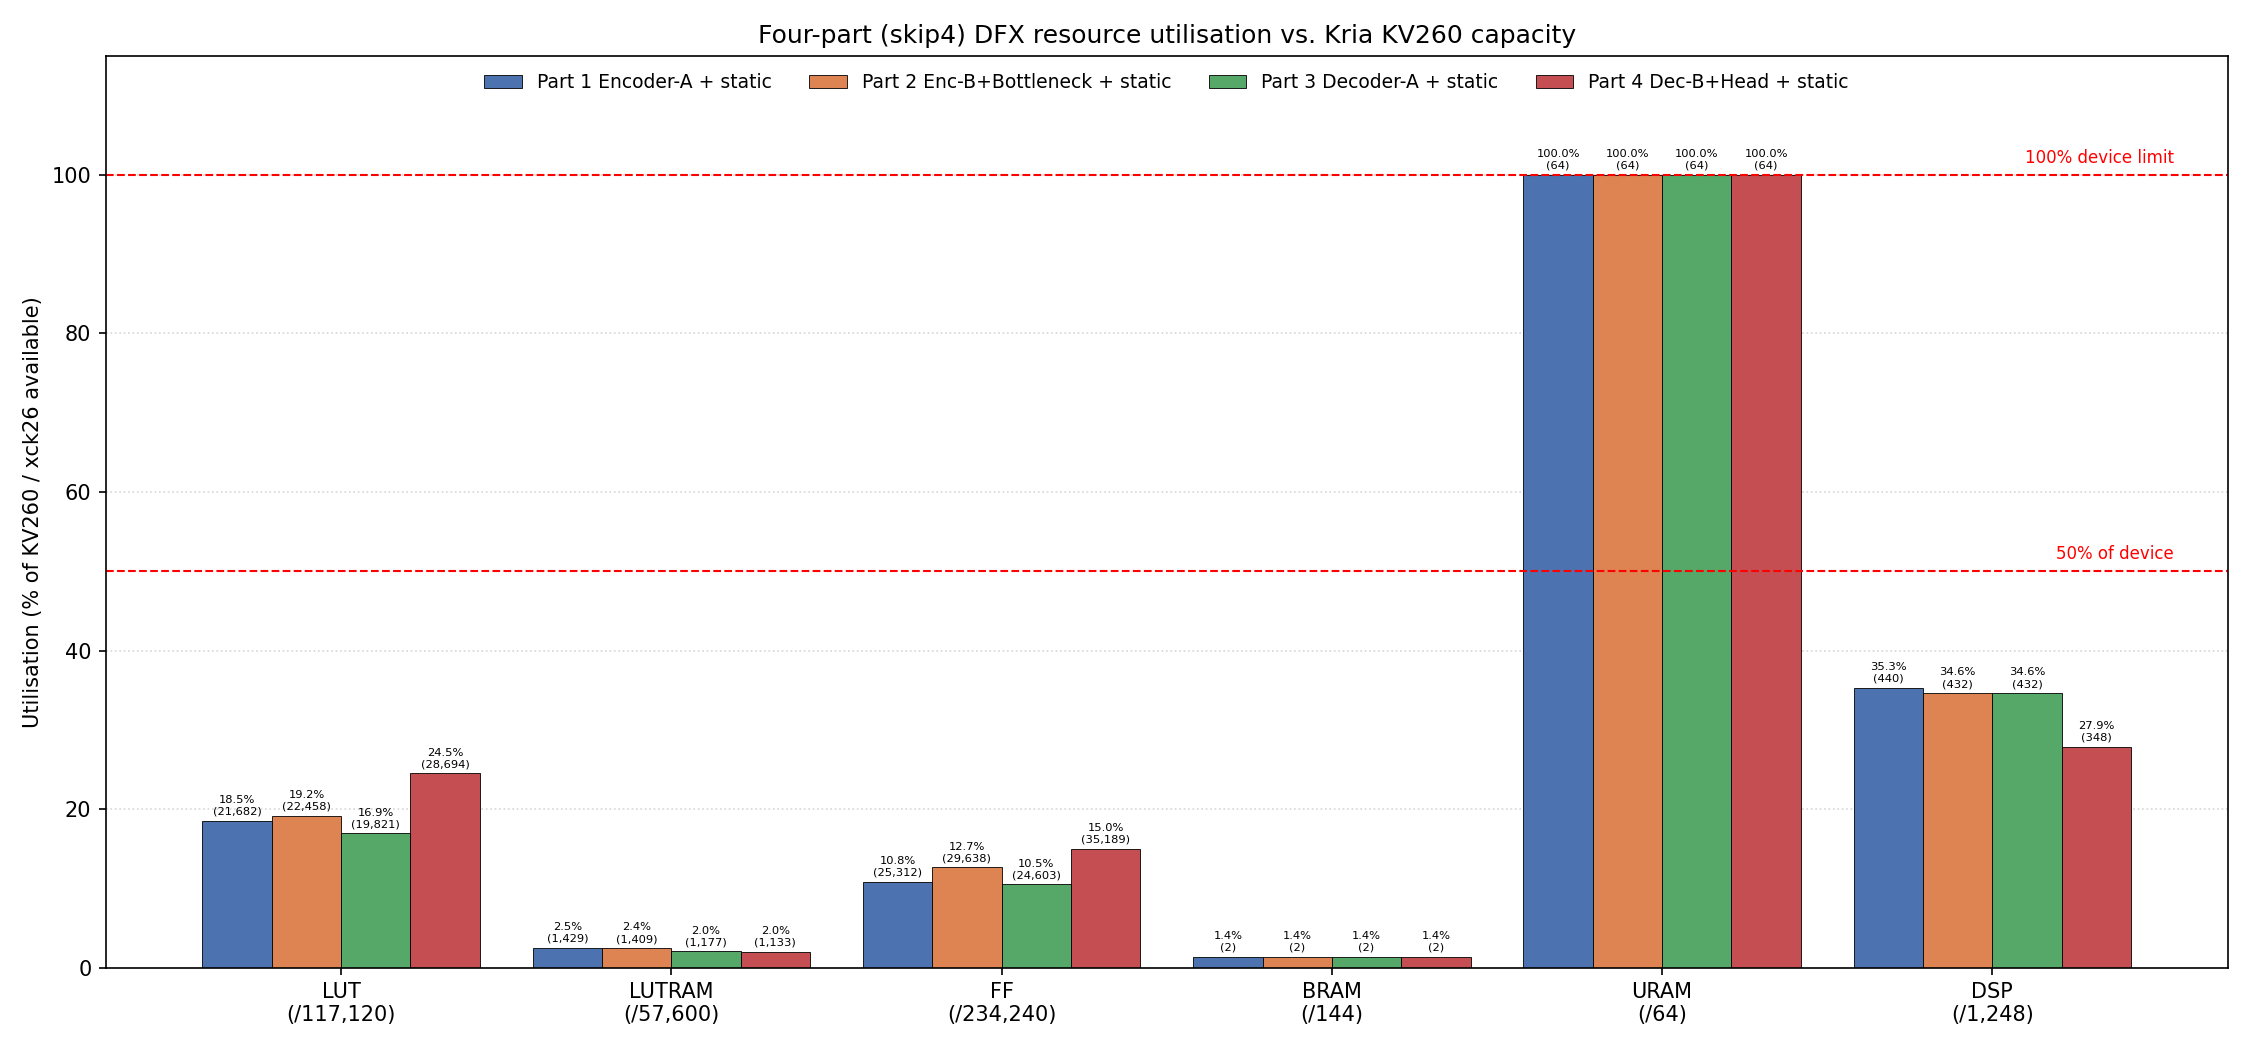
\includegraphics[width=\linewidth,height=\textheight,keepaspectratio]{res/skip4_resource_util.png}
  \caption{Four-part (skip4) resource utilisation per part, as a percentage of the KV260 capacity. Each bar is one RM plus the static region.}
  \label{fig:res_skip4_util}
\end{figure}
\end{landscape}

Apart from URAM (100\%, static streamers), every part stays comfortably below the 50\% per-region line: DSP ranges from \mbox{27.9\% (348)} for Part~4 to \mbox{35.3\% (440)} for Part~1, LUT from \mbox{16.9\% (19\,821)} to \mbox{24.5\% (28\,694)}, and FF from \mbox{10.5\% (24\,603)} to \mbox{15.0\% (35\,189)}; LUTRAM and BRAM stay around 2\% and 1.4\% respectively. The implemented device floorplans in Figure~\ref{fig:fabric_skip4} show the static region (with both PR pblocks empty) and each of the four RMs routed into its region.

\begin{figure}[p]
  \centering
  \begin{subfigure}{0.40\linewidth}
    \centering
    
\includegraphics[width=\linewidth]{fabric/skip4/static_region.png}
    \caption{Static region (both PR pblocks empty).}
  \end{subfigure}

  \vspace{0.5ex}
  \begin{subfigure}{0.43\linewidth}
    \centering
    
\includegraphics[width=\linewidth]{fabric/skip4/rg0_rm0.png}
    \caption{Region 0 / RM 0 — Part 1 (Encoder-A).}
  \end{subfigure}\hfill
  \begin{subfigure}{0.43\linewidth}
    \centering
    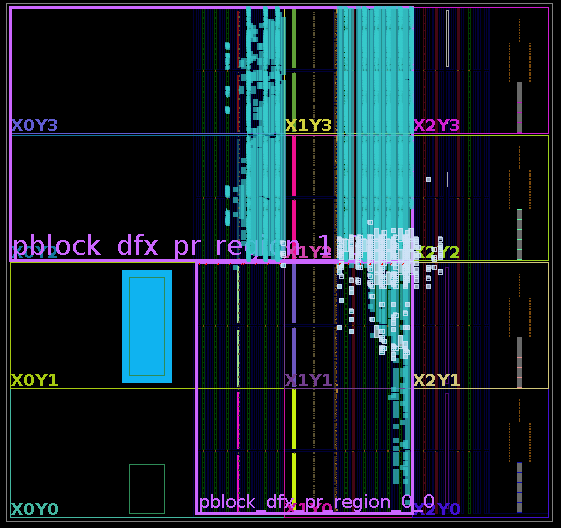
\includegraphics[width=\linewidth]{fabric/skip4/rg1_rm0.png}
    \caption{Region 1 / RM 0 — Part 2 (Encoder-B + Bottleneck).}
  \end{subfigure}

  \vspace{0.5ex}
  \begin{subfigure}{0.43\linewidth}
    \centering
    
\includegraphics[width=\linewidth]{fabric/skip4/rg0_rm1.png}
    \caption{Region 0 / RM 1 — Part 3 (Decoder-A).}
  \end{subfigure}\hfill
  \begin{subfigure}{0.43\linewidth}
    \centering
    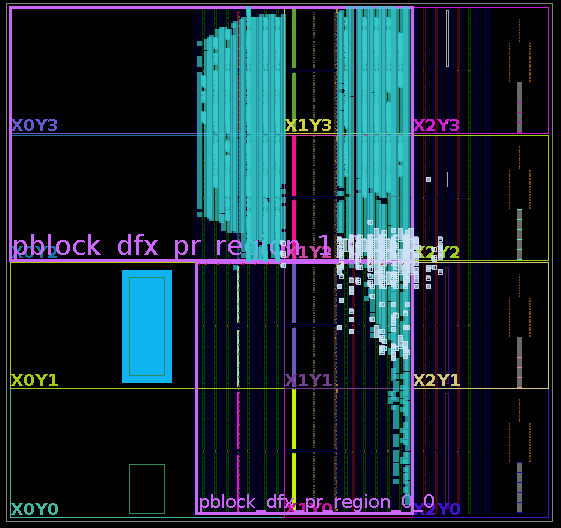
\includegraphics[width=\linewidth]{fabric/skip4/rg1_rm1.png}
    \caption{Region 1 / RM 1 — Part 4 (Decoder-B + Head).}
  \end{subfigure}
  \caption{Four-part scheme: implemented device floorplans of the static region and the four reconfigurable modules across the two PR regions.}
  \label{fig:fabric_skip4}
\end{figure}

\subsubsection{Two-Part Scheme}

In the two-part scheme both halves share a single PR region (\texttt{pblock\_dfx\_pr\_region\_0}) over two phases. Because each half now packs two of the four parts, its per-configuration footprint is roughly double that of the four-part scheme. Figure~\ref{fig:res_skip2_util} reports the utilisation of each half.

\begin{landscape}
\begin{figure}
  \centering
  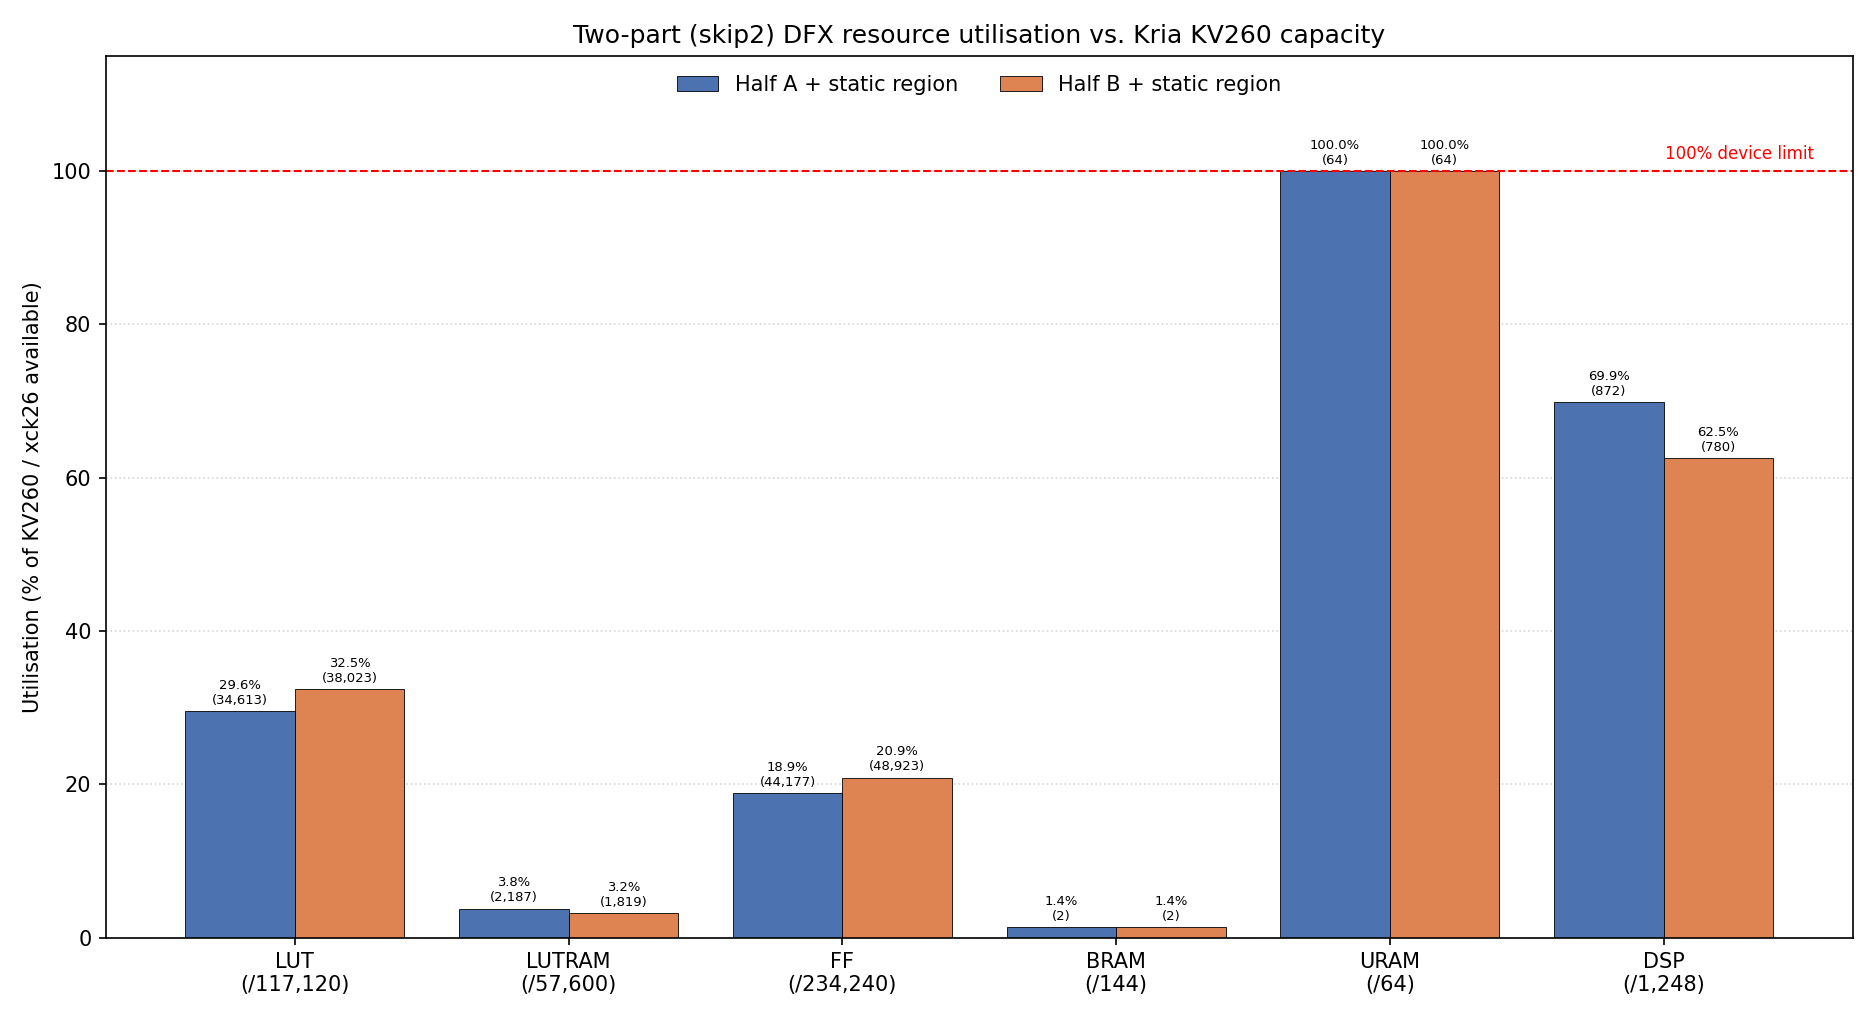
\includegraphics[width=\linewidth,height=\textheight,keepaspectratio]{res/skip2_resource_util.png}
  \caption{Two-part (skip2) resource utilisation per half, as a percentage of the KV260 capacity. Each bar is one RM plus the static region.}
  \label{fig:res_skip2_util}
\end{figure}
\end{landscape}

DSP is now the dominant logic resource, reaching \mbox{69.9\% (872)} for Half~A and \mbox{62.5\% (780)} for Half~B, with LUT at \mbox{29.6\% (34\,613)} / \mbox{32.5\% (38\,023)} and FF at \mbox{18.9\% (44\,177)} / \mbox{20.9\% (48\,923)}; URAM remains at 100\% (static streamers). Compared with the four-part scheme, folding two parts into a single region roughly doubles the LUT/FF/DSP footprint per configuration, trading fabric occupancy for fewer PR regions and fewer reconfiguration phases. The corresponding device floorplans are shown in Figure~\ref{fig:fabric_skip2}.

\begin{figure}[H]
  \centering
  \begin{subfigure}{0.32\linewidth}
    \centering
    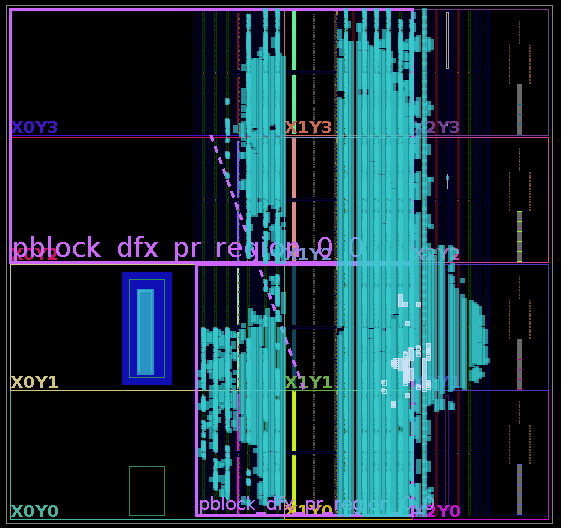
\includegraphics[width=\linewidth]{fabric/skip2/static_region.png}
    \caption{Static region + RM 0 — Half A.}
  \end{subfigure}\hfill
  \begin{subfigure}{0.32\linewidth}
    \centering
    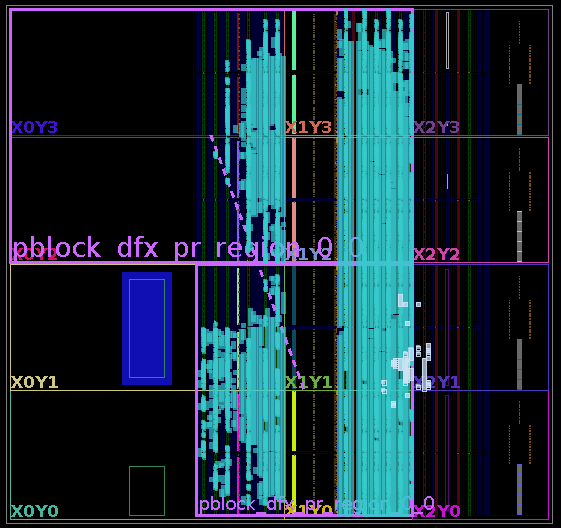
\includegraphics[width=\linewidth]{fabric/skip2/rg0_rm0.png}
    \caption{Region 0 / RM 0 — Half A (encoder + bottleneck).}
  \end{subfigure}\hfill
  \begin{subfigure}{0.32\linewidth}
    \centering
    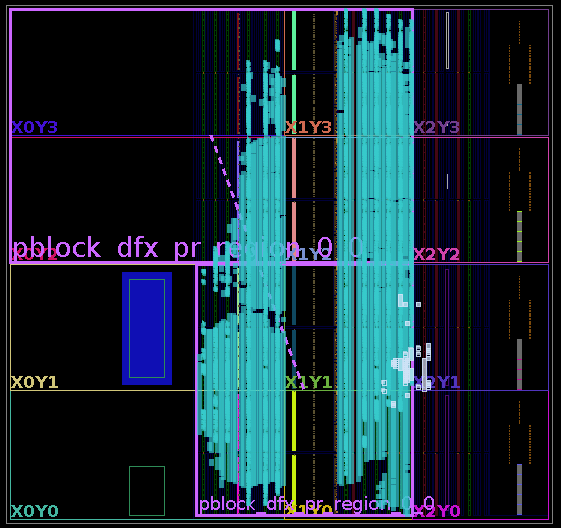
\includegraphics[width=\linewidth]{fabric/skip2/rg0_rm1.png}
    \caption{Region 0 / RM 1 — Half B (decoder + head).}
  \end{subfigure}
  \caption{Two-part scheme: implemented device floorplans of the static region and the two reconfigurable modules in the single PR region.}
  \label{fig:fabric_skip2} 
\end{figure}


\subsection{performance}

We push 900 queries into the both 2-skip and 4-skip model. The timelines below plot these two profiling counters as parallel
lanes: within a slot both lanes start at the same absolute time, and the next
slot starts at the later of the two end times,
$t_{i+1} = t_i + \max(\texttt{recon\_prof}_i, \texttt{exec\_prof}_i)$. Counters
are clock cycles converted to milliseconds at the build clock ($\approx$100~MHz),
and each box is annotated with the PR region / RM variant it drives.

\subsubsection{Four-Part Scheme}

With two PR regions, the four-part scheme is applying latency hiding technique : each slot
reconfigures the \emph{next} region while the \emph{previously} loaded region is
still executing, so the \texttt{recon\_prof} and \texttt{exec\_prof} lanes
overlap in time (Figure~\ref{fig:perf_skip4}).

\subsubsection{Two-Part Scheme}

The two-part scheme folds both halves into a single PR region over two phases,
so reconfiguration and execution cannot overlap: each slot is dominated by one
lane while the other is idle, yielding the serial reconfigure\,$\rightarrow$\,execute
staircase of Figure~\ref{fig:perf_skip2}.

% skip4 and skip2 timelines together on one landscape page
\begin{landscape}
\begin{figure}[H]
  \centering
  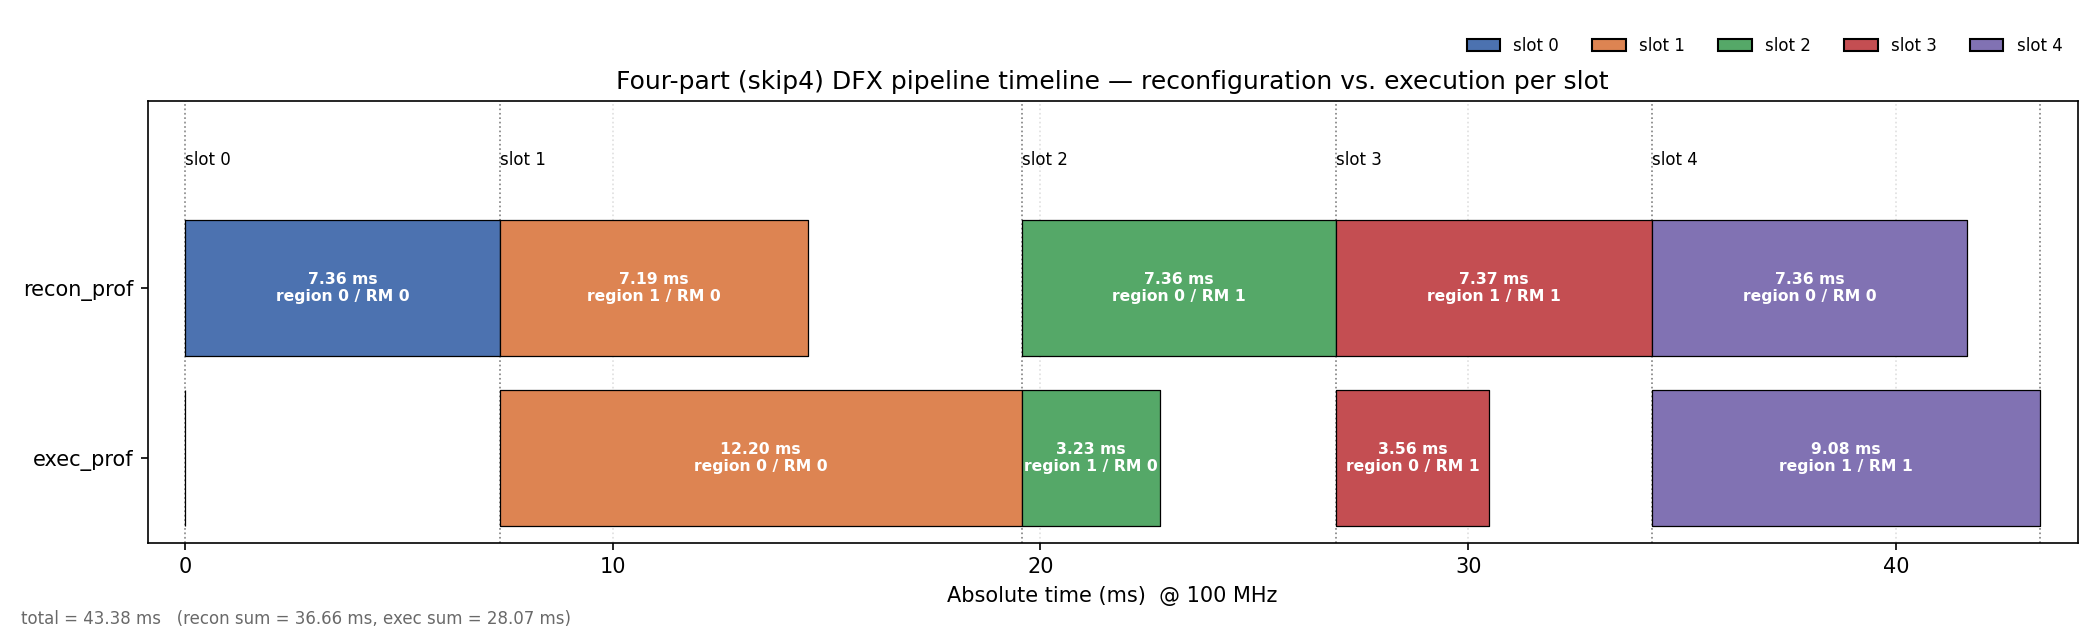
\includegraphics[width=\linewidth,height=0.37\textheight,keepaspectratio]{perf/skip4_perf.png}
  \caption{Four-part (skip4) DFX pipeline timeline: reconfiguration vs.\
  execution per slot. The two regions alternate, overlapping reconfiguration of
  the next region with execution of the current one.}
  \label{fig:perf_skip4}
\end{figure} 

\vspace{0.4cm}

\begin{figure}[H]
  \centering
  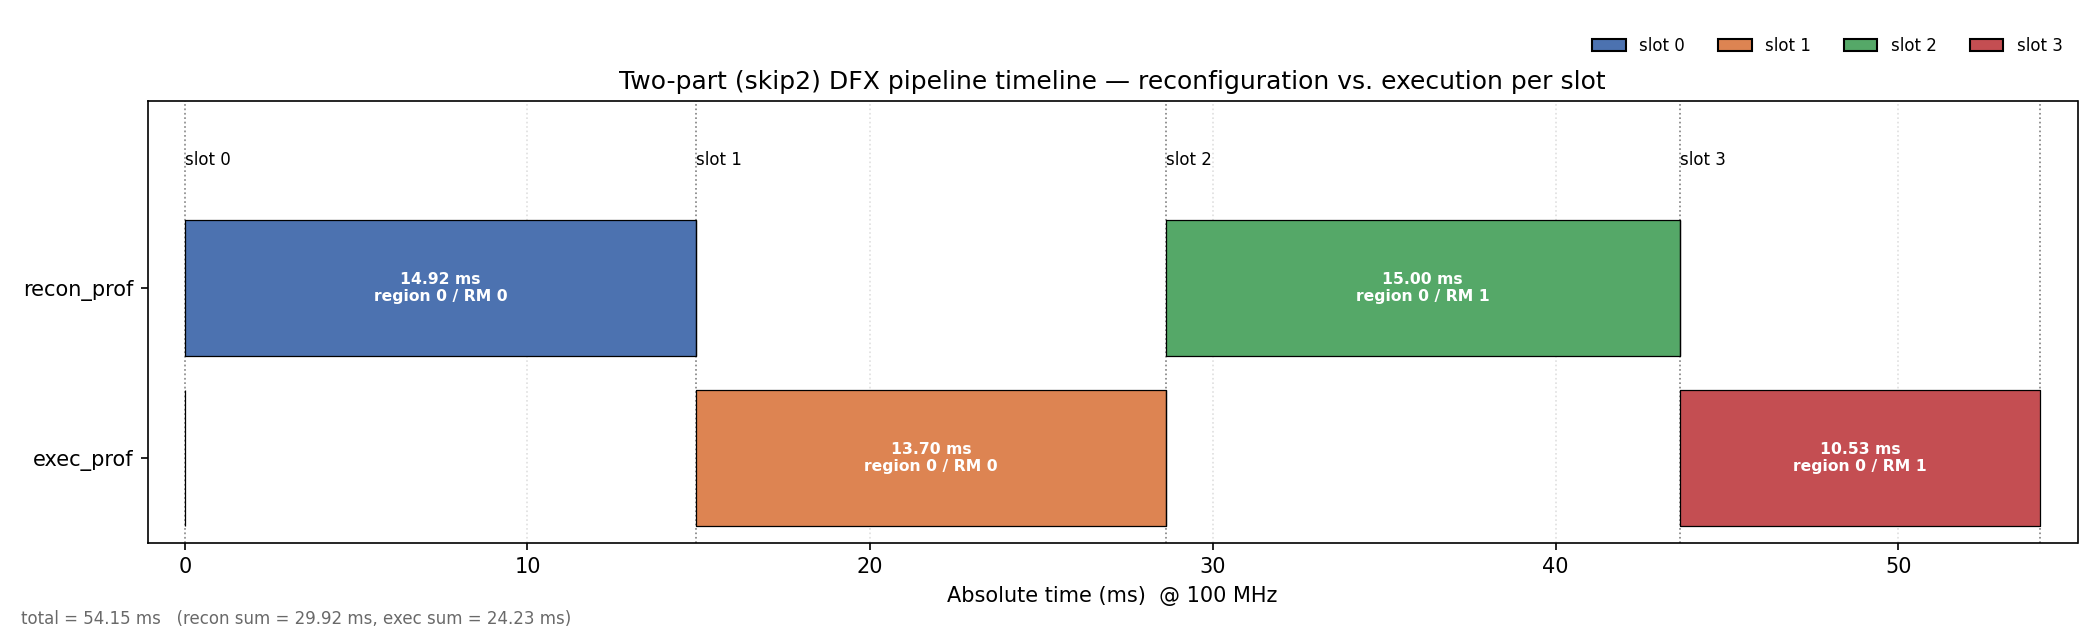
\includegraphics[width=\linewidth,height=0.37\textheight,keepaspectratio]{perf/skip2_perf.png}
  \caption{Two-part (skip2) DFX pipeline timeline: reconfiguration vs.\
  execution per slot. The single shared PR region serialises the two phases.}
  \label{fig:perf_skip2}
\end{figure}
\end{landscape}

\subsubsection{Combined Comparison}

Figure~\ref{fig:perf_combined} overlays both schemes on a common time axis. The
skip2 timeline is shifted so its origin aligns with the start of skip4 slot~1
(skip4 slot~0 will not be considered for performance analysis if the process have been re-execute in the next iteration), letting both
schemes begin real work at the same instant. The overlap saved by
latency-hiding technique is then visible directly: skip4 completes in 3601045 cycles whereas
skip2 runs to 5414838 cycles.

In this calculation, we may conclude that we gain 33.5 \% improvment from the ideal improvment is at 50 \%. The different from the ideal case comes from the unbalance execution time in each session. Morever, we realize that there are DDR4 memory's bandwidth competition in slot 1 (session 1).

\begin{landscape}
\begin{figure}[H]
  \centering
  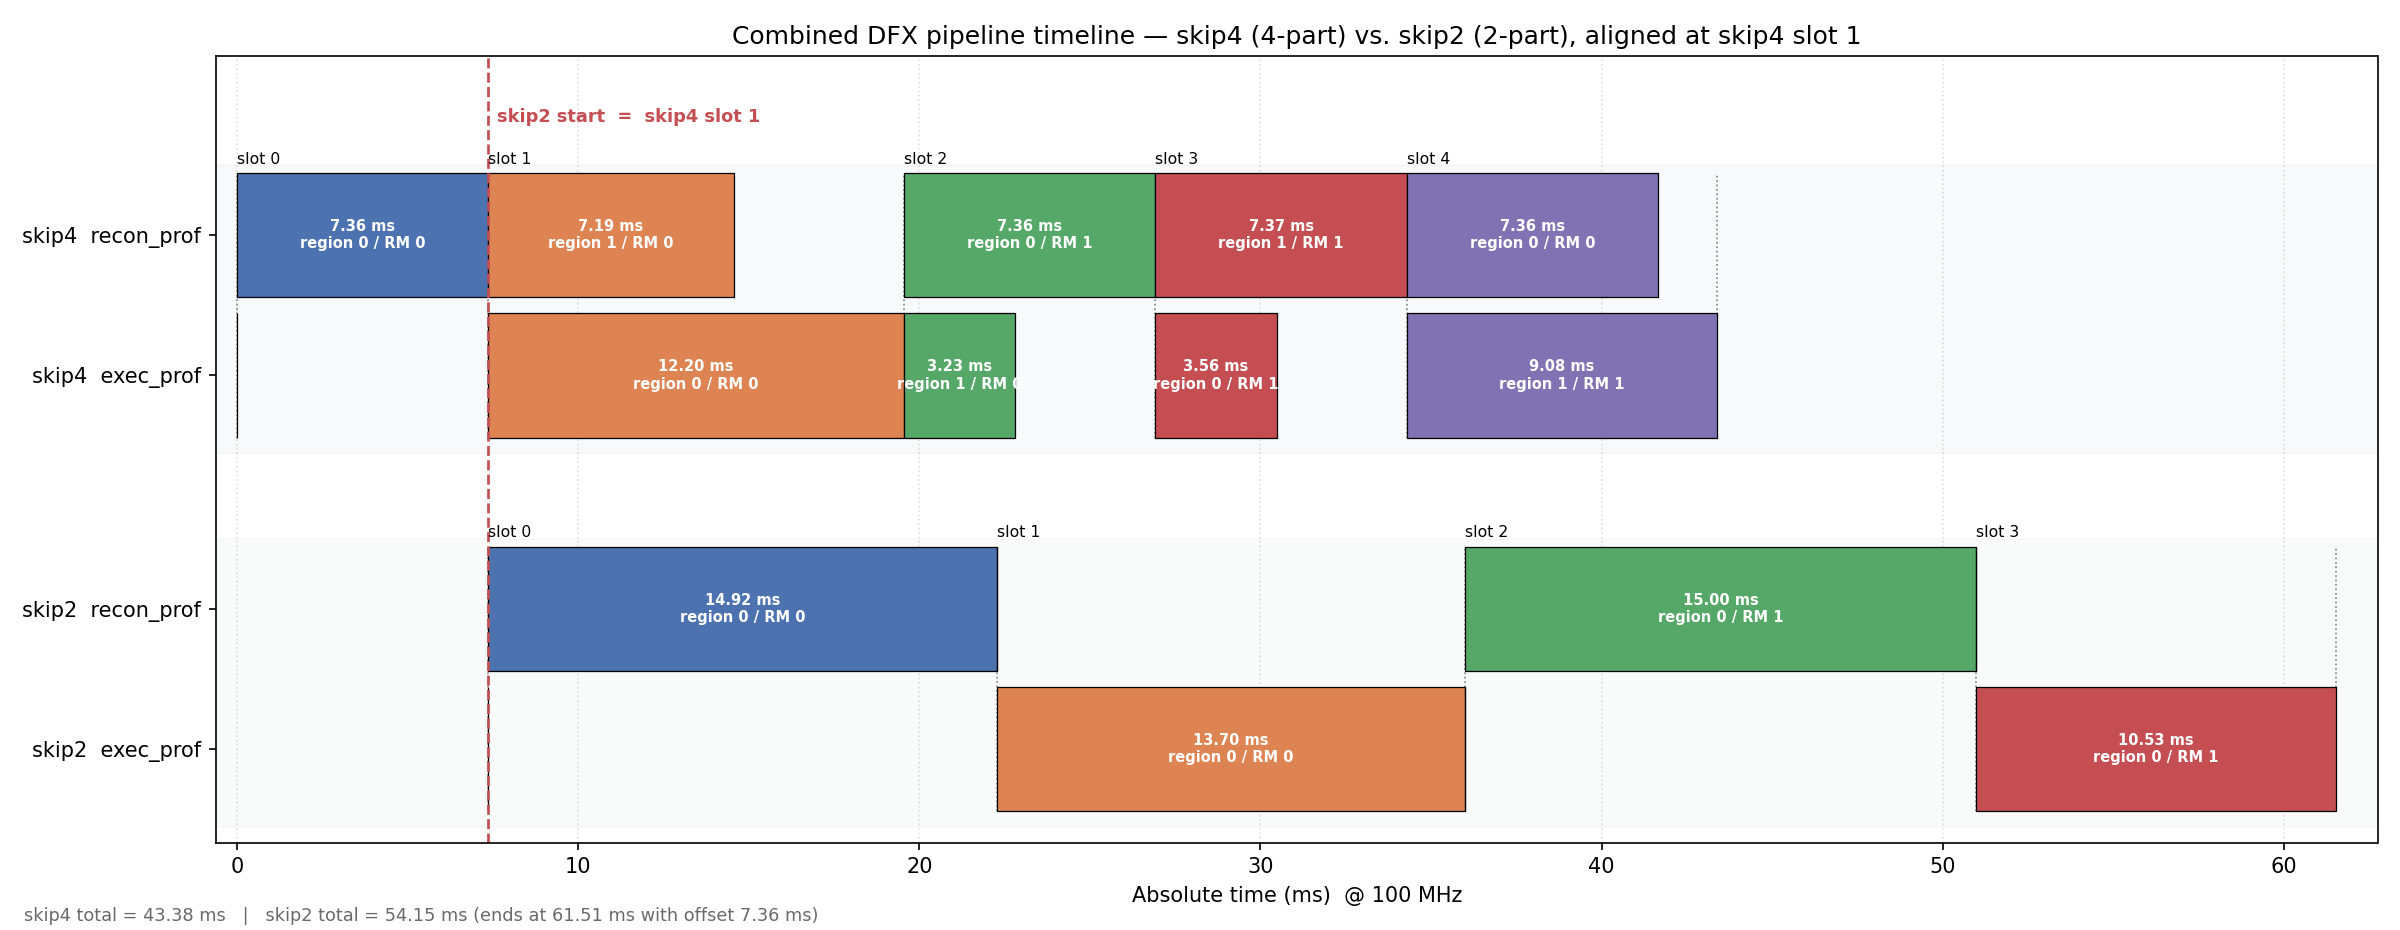
\includegraphics[width=\linewidth,height=0.9\textheight,keepaspectratio]{perf/skip_combined_perf.png}
  \caption{Combined DFX pipeline timeline: four-part (skip4) vs.\ two-part
  (skip2), aligned at skip4 slot~1. The double-buffered skip4 overlaps
  reconfiguration with execution, while the single-region skip2 serialises the
  two phases.}
  \label{fig:perf_combined}
\end{figure}
\end{landscape}

\clearpage

\section{Why DFX4ML? and Its Position}

We got an interesting question from my college that "WHY WE DON'T JUST REPROGRAM ENTIRE FABRIC FOR PARTIAL MODEL AND PUSH QUERIES", and use all DRAM and push many milion of queries at a time so the system will have no reconfigure overhead. (nickname: par-model on full fabric (PMFF))


Therefore, we build the table below to clarify and propose our idea.
\textbf{Note that this comparison is only a conceptual proposal: the entries
reflect our reasoning and expectations, and have not yet been experimentally
verified.}

\begin{table}[H] 
  \centering
  \small
  \caption{Comparison criteria referenced in Table~\ref{tab:dfx4ml_vs_pmff}.}
  \label{tab:dfx4ml_criteria}
  \begin{tabular}{l >{\raggedright\arraybackslash}p{11cm}}
    \toprule
    Name & Criterion \\
    \midrule
    CPU usage       & require CPU for operation \\
    Fabric sharing  & support unrelated system (pid control, communcation chip, network chip, etc.) operating on the same fabric \\
    Latency         & latency (round-trip time when data arrive) \\
    Bulk exec time  & overall exec time (large amount of queries) \\
    Data-hold power & save power by holding data on BRAM/URAM \\
    Skip output BW  & support high bandwidth the data out from the model with multiple skip link \\
    \bottomrule
  \end{tabular}
\end{table} 

\begin{table}[H]
  \centering
  \small
  \caption{DFX4ML (with and without the latency-hiding technique, LH) versus
  par-model on full fabric (PMFF). The criteria names are defined in
  Table~\ref{tab:dfx4ml_criteria}. Green cells mark an outcome that benefits the
  user, yellow cells a moderate outcome, and red cells a drawback.}
  \label{tab:dfx4ml_vs_pmff}
  \begin{tabular}{l
                  >{\centering\arraybackslash}p{2.4cm}
                  >{\centering\arraybackslash}p{2.4cm}
                  >{\raggedright\arraybackslash}p{4.5cm}}
    \toprule
              & \multicolumn{2}{c}{DFX4ML} &      \\
    \cmidrule(lr){2-3}
    Criterion & with LH & without LH & PMFF \\
    \midrule
    CPU usage       & \multicolumn{2}{c}{\cellcolor{green!25}No (only for initialize)} & \cellcolor{red!25}MUST \\
    Fabric sharing  & \multicolumn{2}{c}{\cellcolor{green!25}Yes} & \cellcolor{red!25}NO \\
    Latency         & \cellcolor{green!25}Low & \cellcolor{yellow!40}Moderate & \cellcolor{red!25}High \\
    Bulk exec time  & \cellcolor{yellow!40}Moderate & \cellcolor{red!25}High & \cellcolor{green!25}Low (if not consider DDR4 congestion) \\
    Data-hold power & \multicolumn{2}{c}{\cellcolor{red!25}NO} & \cellcolor{red!25}NO \\
    Skip output BW  & \multicolumn{2}{c}{\cellcolor{green!25}YES} & \cellcolor{red!25}NO \\
    \bottomrule
  \end{tabular}
\end{table}

We explain the key rows of Table~\ref{tab:dfx4ml_vs_pmff} below.

\begin{itemize}
  \item \textbf{CPU usage.} DFX4ML relies on the FPGA's self-reconfiguration,
  so the CPU is involved only during initialization, and even this step could be
  offloaded in a future upgrade so that no CPU is required at all. PMFF, in
  contrast, needs the CPU to reprogram the fabric every time a different partial
  model must be loaded.

  \item \textbf{Latency.} PMFF places a single partial model on the whole fabric
  and executes a large batch of queries at once, so it must wait until enough
  queries have accumulated before it can run. This waiting inflates the
  round-trip latency seen by any individual query. DFX4ML instead processes each
  query as it arrives, keeping latency low.

  \item \textbf{Bulk exec time.} When a very large number of queries is
  processed, DFX4ML can suffer from reconfiguration overhead, because the fabric
  is swapped between model segments; the latency-hiding technique reduces this
  cost but does not remove it. PMFF performs no per-batch reconfiguration, so its
  bulk execution time is low --- provided DDR4 bandwidth congestion is not taken
  into account.

  \item \textbf{Data-hold power.} Our earlier results show that the on-chip
  BRAM/URAM can hold only about 2~MB of data inside the fabric for queries buffering, whereas roughly
  6~MB must be streamed from external memory for each bitstream reconfiguration.
  Because this data cannot be kept entirely on-chip, neither scheme can avoid
  external-memory traffic, and so neither saves power by holding data in
  BRAM/URAM. 
\end{itemize}

\section{Resources}

The code and configurations used in this report are publicly available online:

\begin{itemize}
  \item \textbf{Test model (hls4ml).}\\
  \url{https://github.com/Tanawin1701d/hls4ml/tree/VitisUnifiedPartialExp}
  \item \textbf{DFX4ML --- four-part (skip4) example.}\\
  \url{https://github.com/Tanawin1701d/dfx4ml_infra/blob/7823781813206945127c780cbfc79babe15bd354/example/multi_region_test4}
  \item \textbf{DFX4ML --- two-part (skip2) example.}\\
  \url{https://github.com/Tanawin1701d/dfx4ml_infra/blob/dc4e8507ed2350479570d7c86024793bd4ff18ee/example/multi_region_test5}
\end{itemize}

\section{Next Step}

At present, integrating a model into DFX4ML is a manual process: the HLS4ML IP
must be exported by hand and then imported into the DFX4ML build flow. This
hand-off is workable for a single experiment, but it is tedious and error-prone,
and it does not scale to larger or frequently changing models.

The next step is therefore to bridge the two projects automatically. We plan to
propose a \texttt{vitisUnifiedPartial} backend --- or another suitable
connection mechanism --- that lets HLS4ML emit reconfigurable modules directly
into the DFX4ML partial-reconfiguration flow, removing the manual import step
and providing a seamless path from a trained model to a self-reconfiguring
DFX4ML deployment.

\end{document}
   